\def\assignmenttitle{Modelling and Predicting the Heat Consumption}
\def\assignmentnumber{4}
\def\assignmentdate{17-11-2011}
\def\githuburl{\small\url{https://github.com/alphabits/dtu-fall-2011/tree/master/02417/assignment-4}}
\def\githuburlfoot{\footnotesize\url{https://github.com/alphabits/dtu-fall-2011/tree/master/02417/assignment-4}}

\newcommand\mseven{\seasonal{3,1,3}{0,1,1}{24}}
\newcommand\meight{\seasonal{2,1,2}{0,1,1}{24}}
\newcommand\mnine{\seasonal{1,1,1}{0,1,1}{24}}
\newcommand\mten{\seasonal{3,1,2}{0,1,1}{24}}
\newcommand\meleven{\seasonal{2,1,3}{0,1,1}{24}}
\newcommand\mtwentyone{\seasonal{2,1,1}{0,1,1}{24}}
\newcommand\mtwentytwo{\seasonal{2,1,1}{0,1,2}{24}}
\newcommand\mtwentyeight{\seasonal{2,1,1}{1,1,1}{24}}
\newcommand\tfmtwo{\seasonal{2,1,3}{0,1,2}{24}}

\documentclass[11pt]{article}
\linespread{1}

\renewcommand{\thefootnote}{\fnsymbol{footnote}}

\usepackage{geometry} % see geometry.pdf on how to lay out the page. There's lots.
\usepackage[utf8]{inputenc}
\usepackage[T1]{fontenc}
\usepackage{array}
\usepackage{amsmath,amssymb,latexsym,epic,eepic,epsfig,graphics,psfrag}
\usepackage{amsfonts}
\usepackage{graphicx,float}
\usepackage{color}
\definecolor{mygray}{RGB}{244,244,244}
\definecolor{gray}{gray}{0.5}
\definecolor{myredish}{RGB}{193,33,97}
\definecolor{grayblue}{RGB}{91,112,142}
\definecolor{myorange}{RGB}{255,134,0}
\definecolor{green}{rgb}{0,0.4,0}

\usepackage[english]{babel}

\usepackage[bottom]{footmisc}

\usepackage{fancyhdr}
\pagestyle{fancy}
\lhead{\small\textit{Assignment \assignmentnumber -- 02417 Time Series Analysis -- Anders Hørsted (s082382)}}
\rhead{\thepage}
\chead{}
\lfoot{}\cfoot{}\rfoot{}

\usepackage{subfigure}
\usepackage{pstricks}
\usepackage{pst-node}
\usepackage{wrapfig}
\usepackage{caption}
\usepackage{multirow}
%\usepackage{fouriernc}
%\usepackage[charter]{mathdesign}
\usepackage{lmodern}
\usepackage[normalem]{ulem}
\geometry{a4paper} % or letter or a5paper or ... etc
% \geometry{landscape} % rotated page geometry

\usepackage{url}


\makeatletter
\renewcommand*\env@matrix[1][*\c@MaxMatrixCols c]{%
  \hskip -\arraycolsep
  \let\@ifnextchar\new@ifnextchar
  \array{#1}}
\makeatother

\newcommand\myimp{\quad\Leftrightarrow\quad}
\newcommand\half{\frac{1}{2}}
\newcommand\myvec[1]{\mathbf{#1}}
\newcommand\mymod[1]{\ (\text{mod }#1)}
\newcommand\myreal{\mathbb{R}}
\newcommand\mynatural{\mathbb{N}}
\newcommand\myinteger{\mathbb{Z}}
\newcommand\mycomplex{\mathbb{C}}
\newcommand\myint{\text{int}}
\newcommand\norm[1]{||\,#1\,||}
\newcommand\bignorm[1]{\big|\big|\,#1\,\big|\big|}
\newcommand\seq[1]{\big\{#1\big\}}
\newcommand\smallseq[1]{\{#1\}}
\newcommand\smallseqtoinf[1]{\smallseq{#1}_{k=1}^\infty}
\newcommand\lonew{\ell^1_w}
\newcommand\lone{\ell^1}
\newcommand\ltwo{\ell^2(\mynatural)}
\newcommand\ip[2]{\langle#1,#2\rangle}
\newcommand\hilbert[1]{\mathcal{#1}}
\newcommand\uinf{u_{\infty}}
\newcommand\erf{\text{erf\,}}
\newcommand\infint{\int_{\infty}^{\infty}}
\newcommand\fpi{FPI}
\newcommand\E[1]{\text{E}[#1]}
\newcommand\Var[1]{\text{Var}[#1]}
\newcommand\Cov[1]{\text{Cov}[#1]}
\newcommand\myverb[1]{{\footnotesize\texttt{#1}}}
\newcommand\Yhat{\widehat{Y}}
\newcommand\given{\,|\,}

\usepackage[scaled]{beramono}
\usepackage{listings}
\lstset {                 % A rudimentary config that shows off some features.
    language=R,
    basicstyle=\scriptsize\ttfamily, % Without beramono, we'd get cmtt, the teletype font.
    commentstyle=\textit, % cmtt doesn't do italics. It might do slanted text though.
    keywordstyle=,
    identifierstyle=,
    framextopmargin=4pt,
    framexbottommargin=4pt,
    framexleftmargin=4pt,
    framexrightmargin=4pt,
    xleftmargin=4pt,
    xrightmargin=4pt,
    backgroundcolor=\color{mygray},
    frame=single,
    showstringspaces=false,
    captionpos=b,
    tabsize=4            % Or whatever you use in your editor, I suppose.
}

\renewcommand{\lstlistlistingname}{Code Listings}
\renewcommand{\lstlistingname}{Code Listing}

\usepackage{tabulary}
\newcolumntype{y}{>{\centering\arraybackslash}R}

\title{\assignmenttitle}
\date{\assignmentdate}
\author{Assignment \assignmentnumber\ -- 02417 Time Series Analysis -- Anders Hørsted (s082382)}
%\author{}
\date{} % delete this line to display the current date



%%% BEGIN DOCUMENT
\begin{document}

\maketitle

In this report models describing the heat consumption in the VEKS system are
build. As data for the models, a year of hourly measurements of the heat
consumption along with various climate variables are given. First a simple
model, based only on the heat consumption measurements, is build. Then a more
complex model that incorporates information from the climate data is build. For
both models 1- and 6-hour predictions of the heat consumption are made and the
performance is checked by comparing the predictions with the actual values.

\section*{Building the simple model}

In the simple model only the data of past heat consumption is used. First the
data is plotted and shown in figure~\ref{fig:hc-ts}.

\begin{figure}[ht]
    \centering
    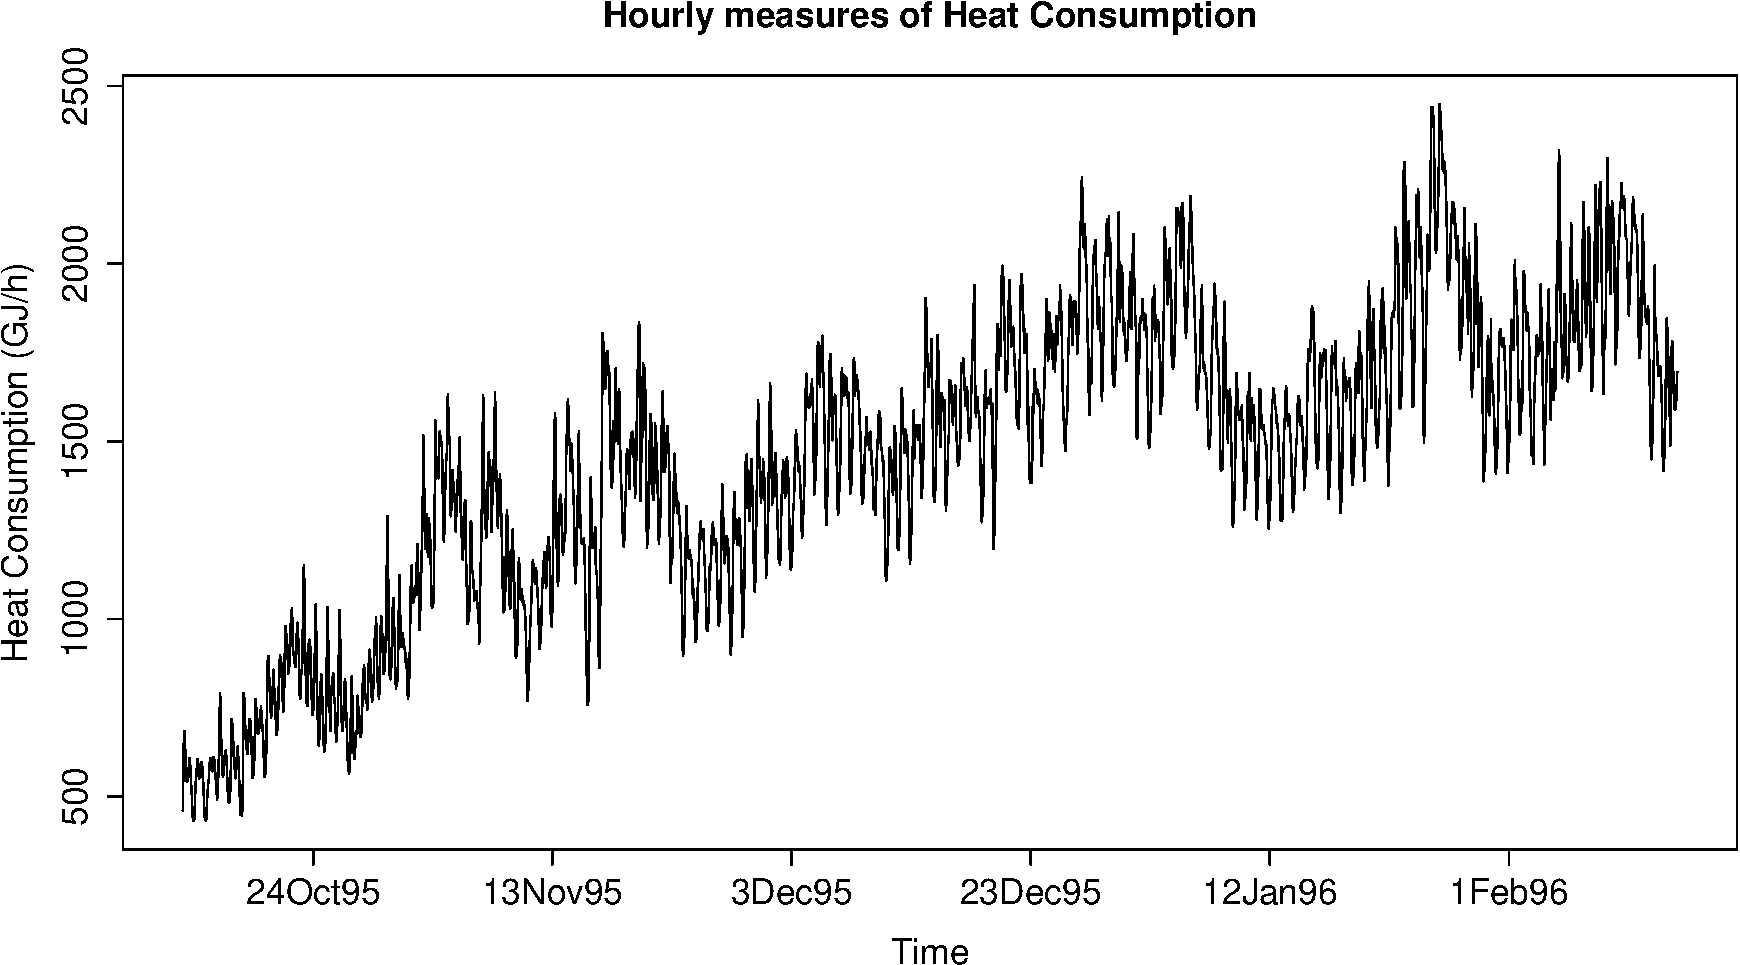
\includegraphics[width=120mm]{../plots/hc-ts.pdf}
    \caption{Heat Consumption time series}
    \label{fig:hc-ts}
\end{figure}

From the plot an upward trend is seen and high frequency oscillations are also
noticed. Also it looks as if the variance increases along with the time. To look into this a range-mean plot is created and shown in figure~\ref{fig:range-mean}. 

\begin{figure}[ht]
    \centering
    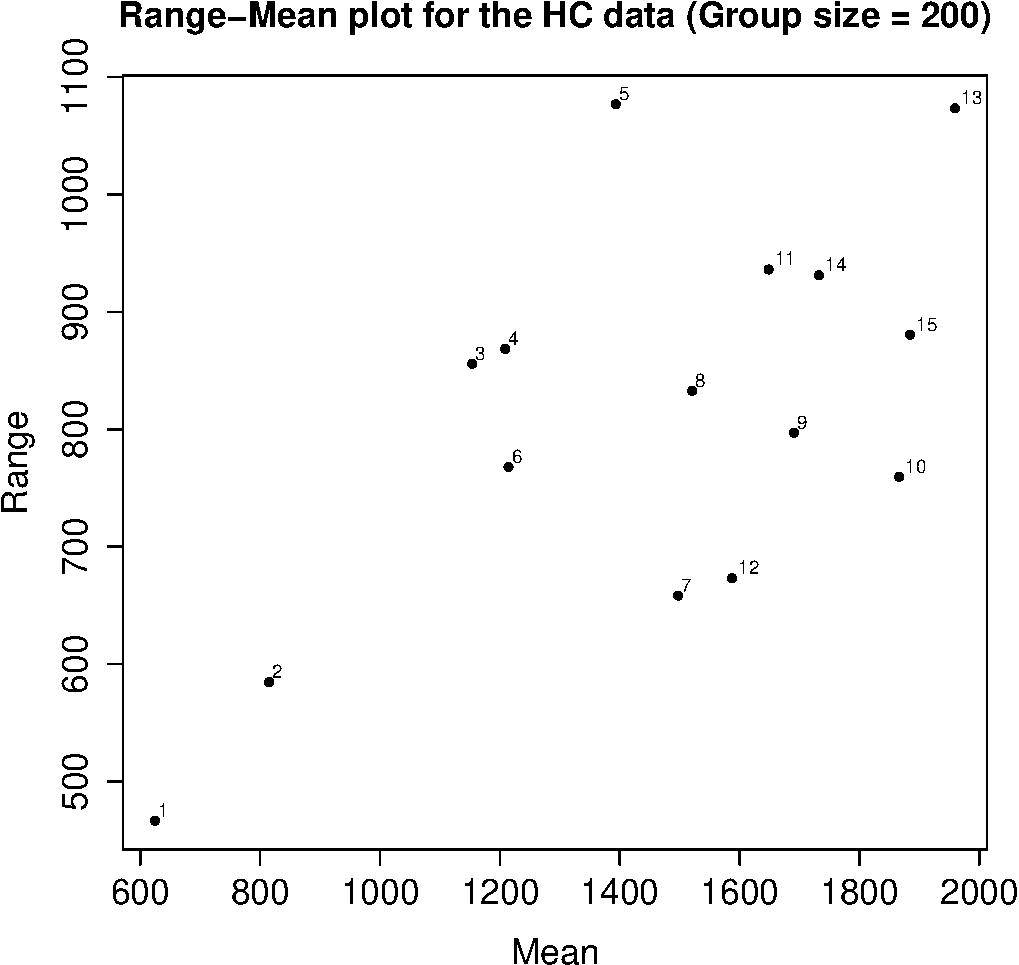
\includegraphics[width=70mm]{../plots/range-mean-plot.pdf}
    \caption{Range-Mean plot for the Heat Consumption series}
    \label{fig:range-mean}
\end{figure}

Although a linear trend can be seen in the range-mean plot, most groups are gathered in what seems to be a random cluster. Only group 1 and 2 have lower means. The conclusion is that the original data is not transformed. 

To further investigate the data the \acf\ and the \pacf\ for the heat
consumption series are plotted and shown in figure~\ref{fig:hc-acfs}.

\begin{figure}
    \centering
    \mbox{\subfigure{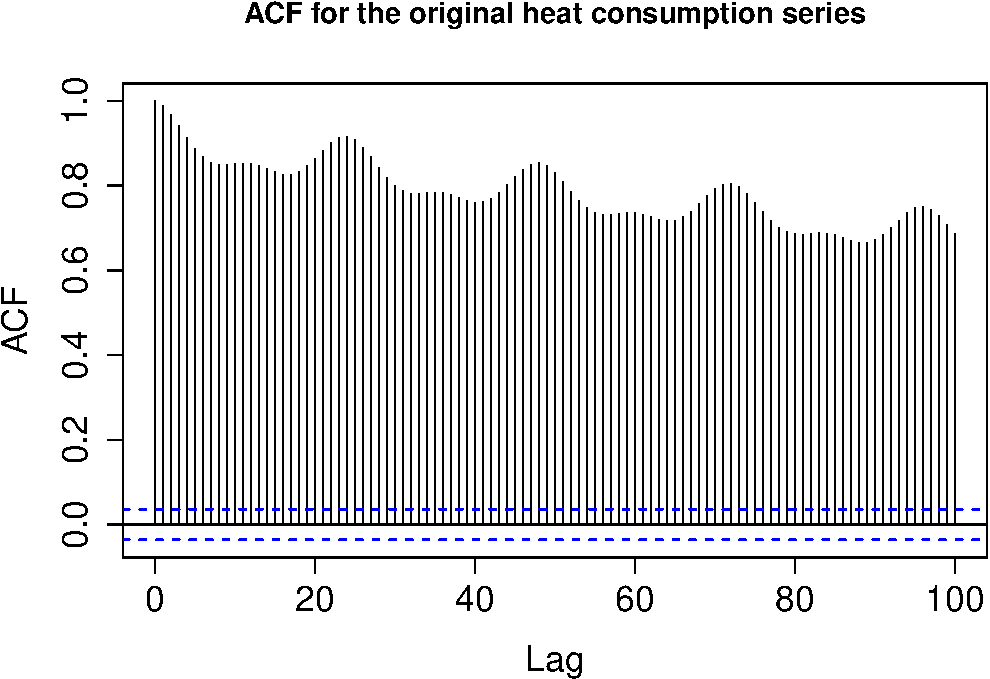
\includegraphics[width=70mm]{../plots/acf-hc.pdf}} \quad 
          \subfigure{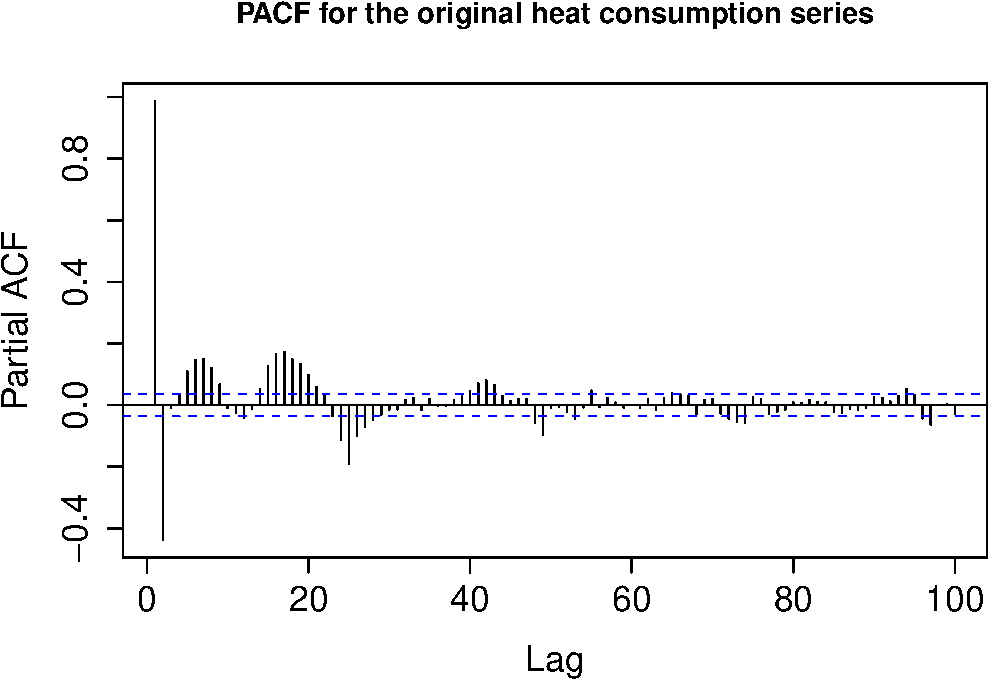
\includegraphics[width=70mm]{../plots/pacf-hc.pdf}}}
    \caption{\acf\ and \pacf\ for the Heat Consumption series}
    \label{fig:hc-acfs}
\end{figure}

From the \acf\ it is seen that the series is non-stationary. Also a seasonallity with period 24 is seen. This isn't surprising since the series consists of hourly measurements. The \pacf\ is numerically large for lag 1, and for higher lags it looks a bit like a damped sine function. 

\subsection*{Removing the non-stationarity}

The first problem to tackle is the non-stationarity. To remove the upward trend the original series $Y_t$ is differenced once

\begin{equation*}
    W_t = \nabla Y_t
\end{equation*}

This gives the new series $W_t$ and the \acf\ and \pacf\ for this series are shown in figure~\ref{fig:hc-diff-acfs}.

\begin{figure}
    \centering
    \mbox{\subfigure{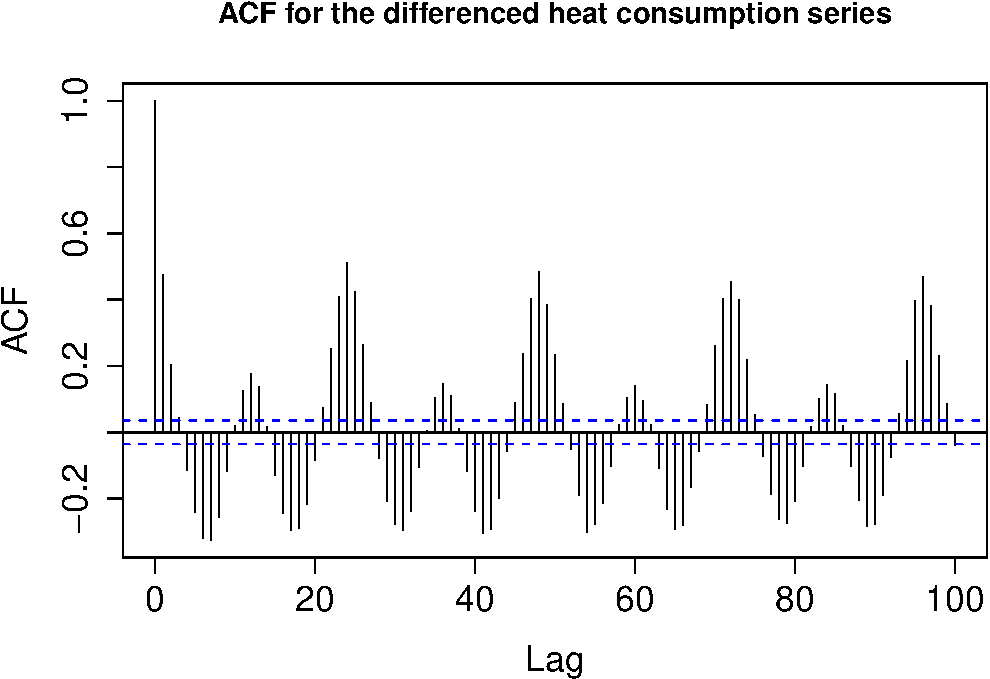
\includegraphics[width=70mm]{../plots/acf-hc-diff.pdf}} \quad 
          \subfigure{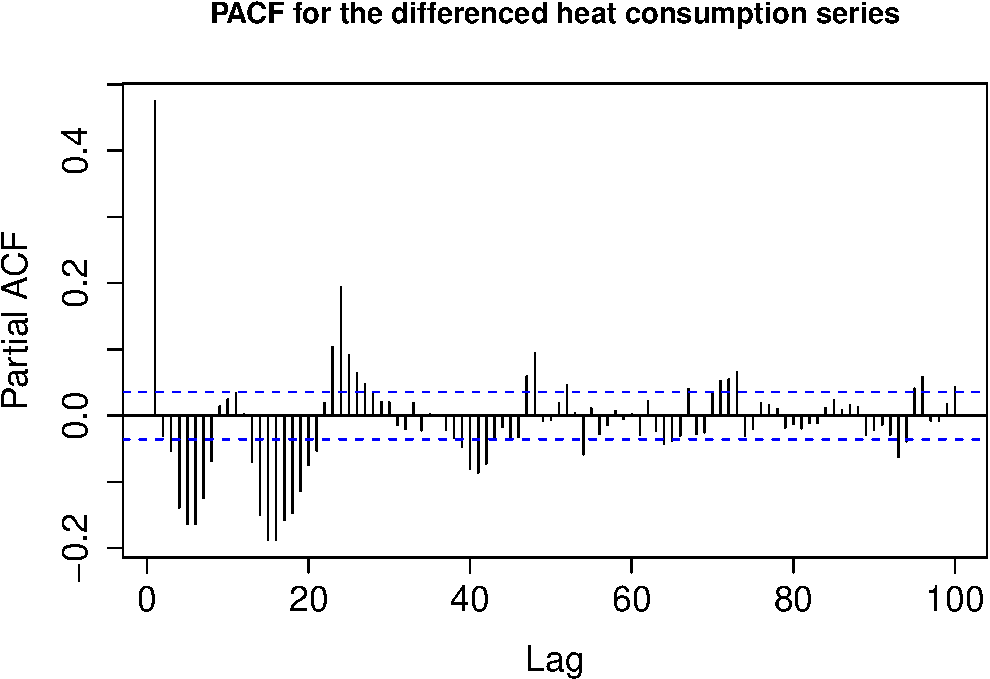
\includegraphics[width=70mm]{../plots/pacf-hc-diff.pdf}}}
    \caption{\acf\ and \pacf\ for the differenced Heat Consumption series}
    \label{fig:hc-diff-acfs}
\end{figure}

A lot of the correlation is gone for some of the lags, but there are still
something to be removed. The \acf\ have some distinct patterns of spikes, that
are separated by 24 lags. It therefore seems like a good idea to do a seasonal
difference with period 24 on the $W_t$ series. This gives

\begin{equation*}
    Z_t = \nabla_{24}W_t = \nabla\nabla_{24} Y_t
\end{equation*}

The \acf\ and \pacf\ for this new series is calculated and shown in
figure~\ref{fig:hc-diff-seasonal-acfs}. A lot of the remaining correlation is
gone. In the \acf\ the first 5 lags and the 24'th lag are different from zero.
In the \pacf\ the first 5 or 6 lags are different from zero, and then the lags
that are a multiplum of 24 seems to slowly decay. Also two or three lags around
the lags that are a multiplum of 24, are seen to be different from zero. These
observations indicates that we probably need a non-seasonal ARMA$(p,q)$ model
and to get started we choose $p=q=3$. For the seasonal correlations only the
first lag (lag 24) is different from zero in the \acf\ and the seasonal lag
slowly decays in the \pacf. This indicates that a seasonal MA(1) should be
appropriate. The first model we are trying to fit to the $Y_t$ series is
therefore a multiplicative $(3,1,3)\times(0,1,1)_{24}$ seasonal model.

\begin{figure}
    \centering
    \mbox{\subfigure{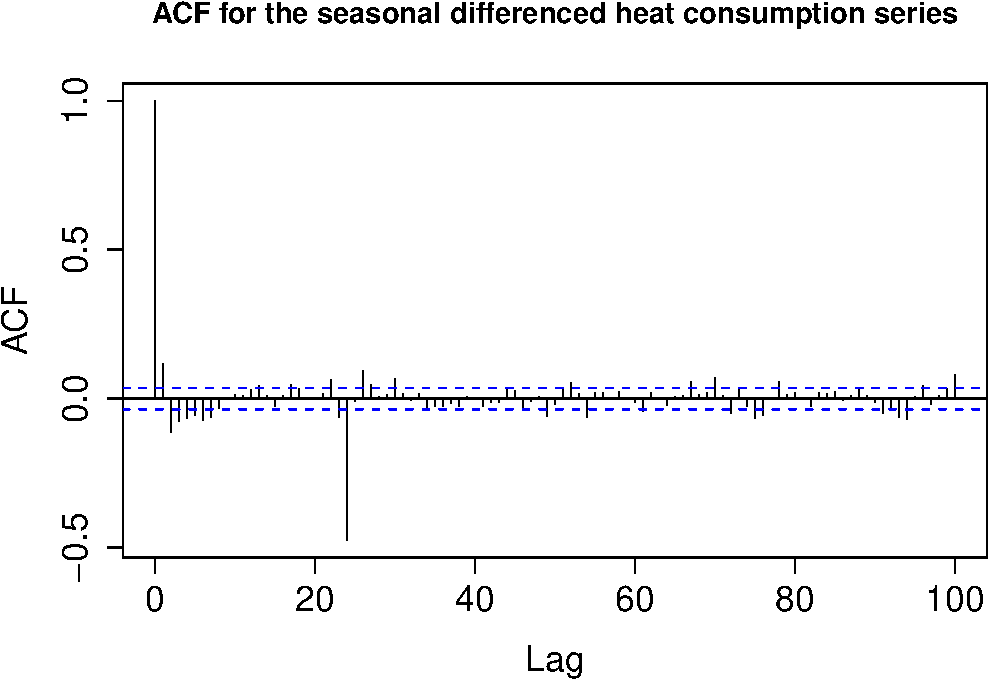
\includegraphics[width=70mm]{../plots/acf-hc-diff-season.pdf}} \quad 
          \subfigure{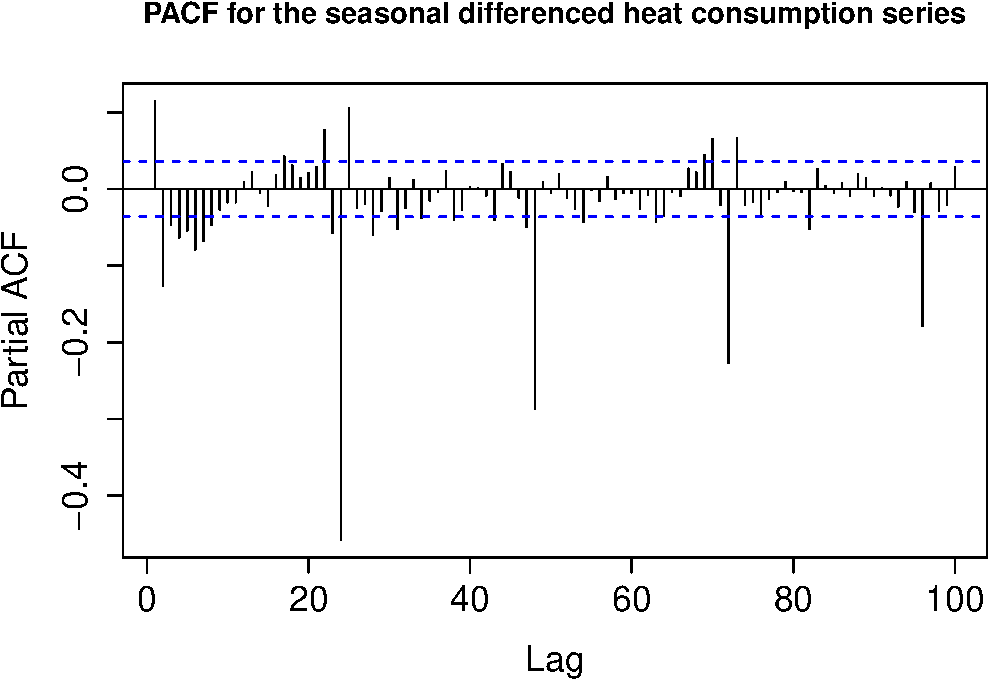
\includegraphics[width=70mm]{../plots/pacf-hc-diff-season.pdf}}}
    \caption{\acf\ and \pacf\ for the combined differenced and seasonal diffirenced Heat Consumption series}
    \label{fig:hc-diff-seasonal-acfs}
\end{figure}

\FloatBarrier

\subsection*{Fitting the $(3,1,3)\times(0,1,1)_{24}$ model}

A \seasonal{3,1,3}{0,1,1}{24} model is fitted and the summary along with the \acf\ and \pacf\ of the residuals are shown in figure~\ref{fig:m7-summary}.

\begin{figure}[!htb]
    \centering
    \mbox{\subfigure{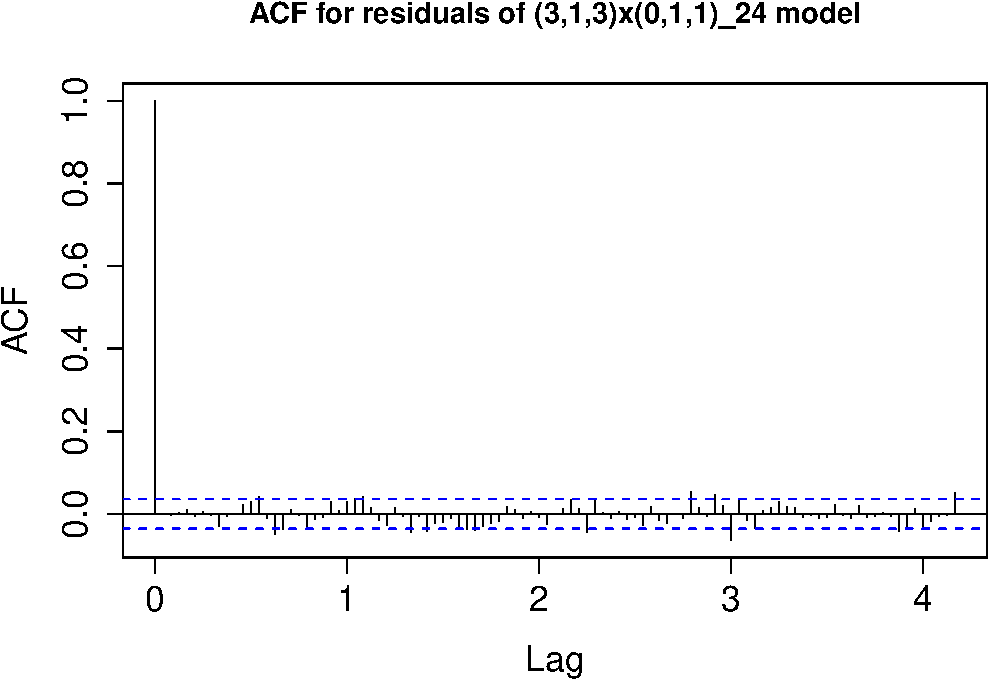
\includegraphics[width=70mm]{../plots/m7-residual-acf.pdf}} \quad 
          \subfigure{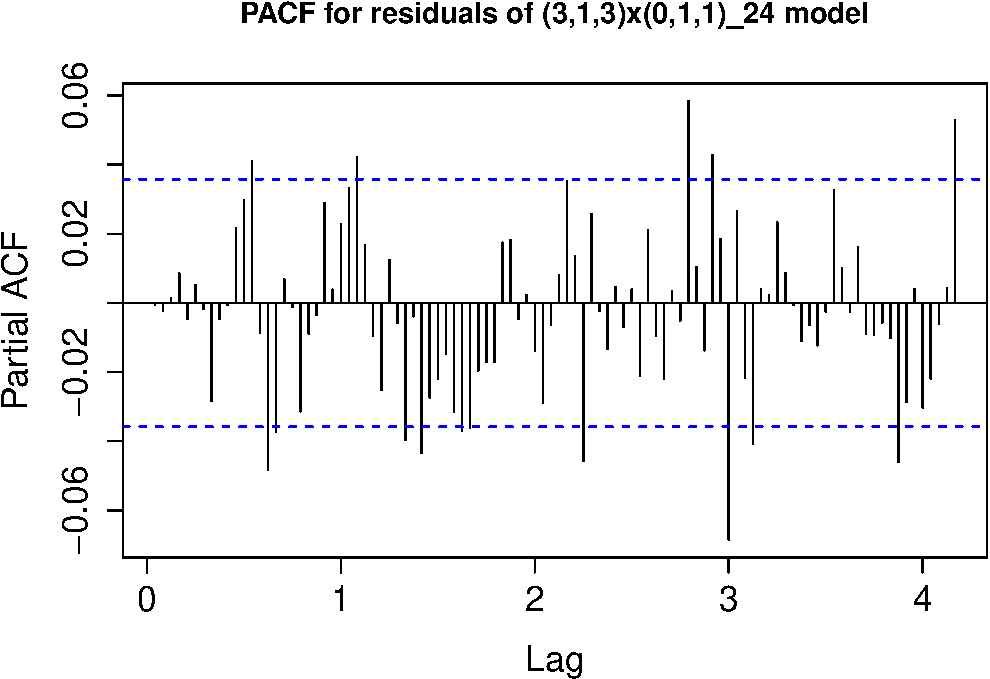
\includegraphics[width=70mm]{../plots/m7-residual-pacf.pdf}}}
    \parbox{.8\textwidth}{\lstinputlisting[firstline=5,lastline=10]{../tables/m7-summary.txt}}
    \caption{The \acf\ and \pacf\ for the residuals of the \mseven\ model}
    \label{fig:m7-summary}
\end{figure}

It is seen that the model fit isn't perfect. For a well fit model the residuals should be white noise and therefore the \acf\ and \pacf\ should show no significant correlation for lags greater than zero. Especially lag 72 in both the \acf\ and \pacf\ is significantly greater than zero. This could hint that we somehow need a seasonal AR part. But first we try to simplify the non-seasonal ARMA model. This will probably give good results since many of the coefficients in the \seasonal{3,1,3}{0,1,1}{24} model is not significantly different from zero. 

\subsection*{The \mten\ and \meleven\ model}

The model from the previous section is tried simplified by decreasing the nonseasonal AR- and MA-part separately. The results from fitting the \mten\ and \meleven\ models are shown in \appref{m10-m11}. The \acf\ and \pacf\ is almost identical to the \mseven model and the AIC score increases for both model. We therefore continue and tries the simpler \meight\ model.

\subsection*{The \meight\ model}

Fitting the \meight\ model gives the summary and \acf/\pacf\ shown in figure~\ref{fig:m8-summary}. 

\begin{figure}[!htb]
    \centering
    \mbox{\subfigure{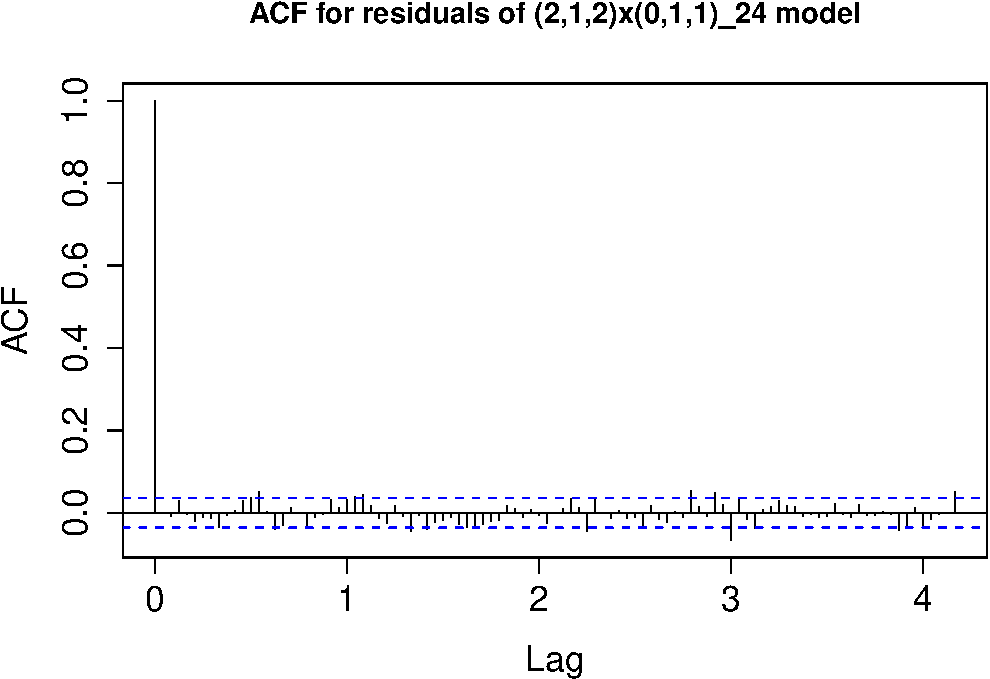
\includegraphics[width=70mm]{../plots/m8-residual-acf.pdf}} \quad 
          \subfigure{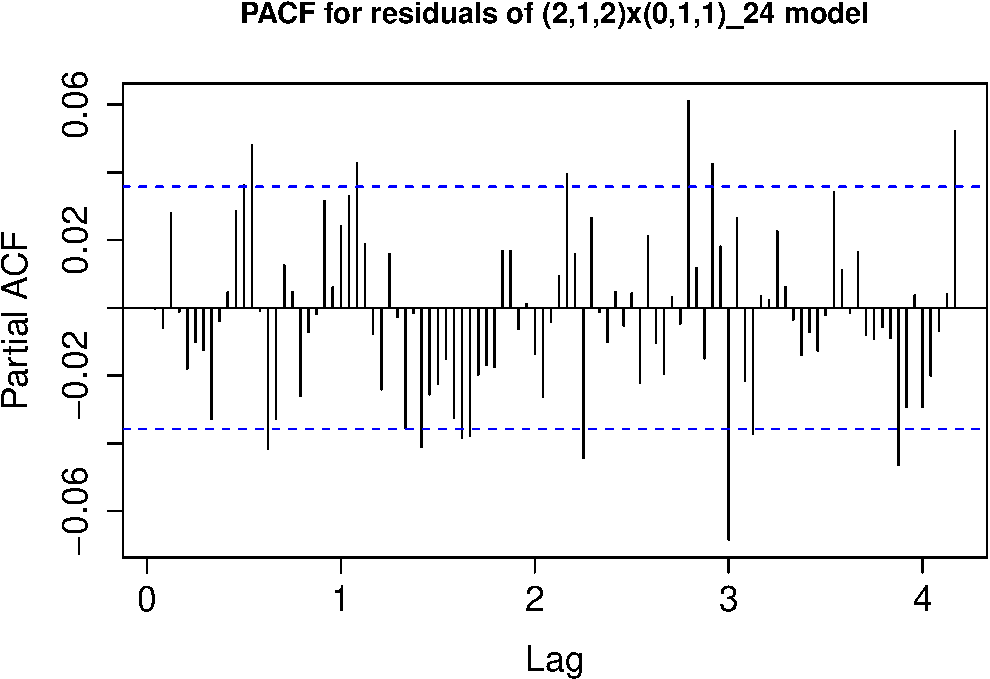
\includegraphics[width=70mm]{../plots/m8-residual-pacf.pdf}}}
    \parbox{.8\textwidth}{\lstinputlisting[firstline=5,lastline=10]{../tables/m8-summary.txt}}
    \caption{The \acf\ and \pacf\ for the residuals of the \meight\ model}
    \label{fig:m8-summary}
\end{figure}

The \acf\ and \pacf\ still looks almost identical to the \mseven\ model and the AIC score has only increase a little. Since this new model is simpler it seems more appropriate to use when we should try to make the seasonal part more complex. Looking at the R summary for this new model it is seen that the coefficient for the second order MA term is not significantly different from zero. Therefore we try to fit the even simpler \mtwentyone\ model.

\subsection*{The \mtwentyone\ model}

The \mtwentyone\ model is fitted and gives the results shown in figure~\ref{fig:m21-summary}.

\begin{figure}[!htb]
    \centering
    \mbox{\subfigure{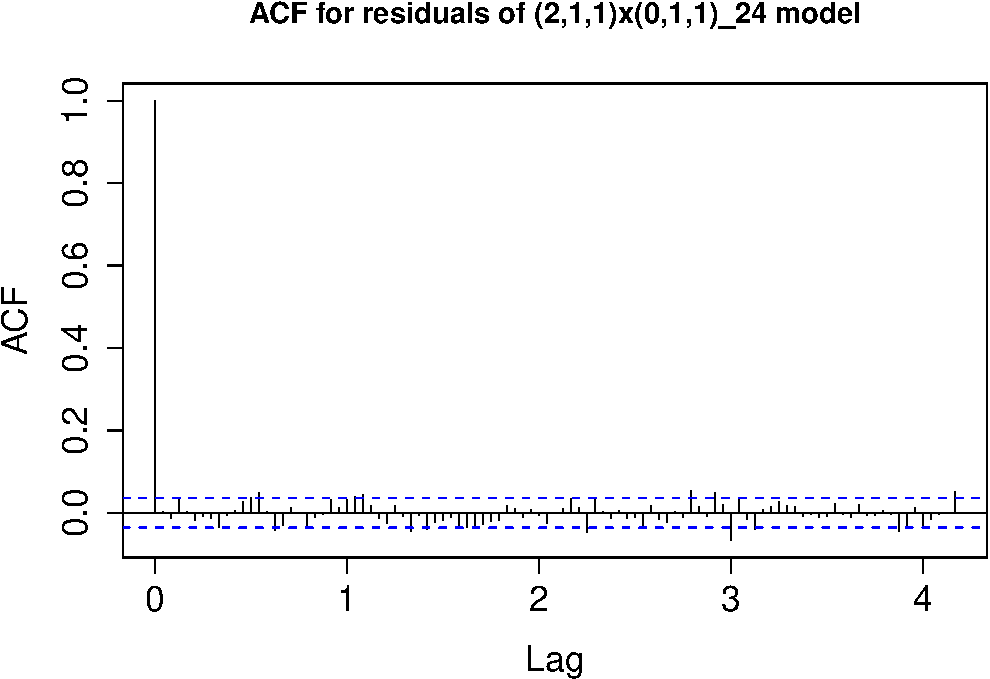
\includegraphics[width=70mm]{../plots/m21-residual-acf.pdf}} \quad 
          \subfigure{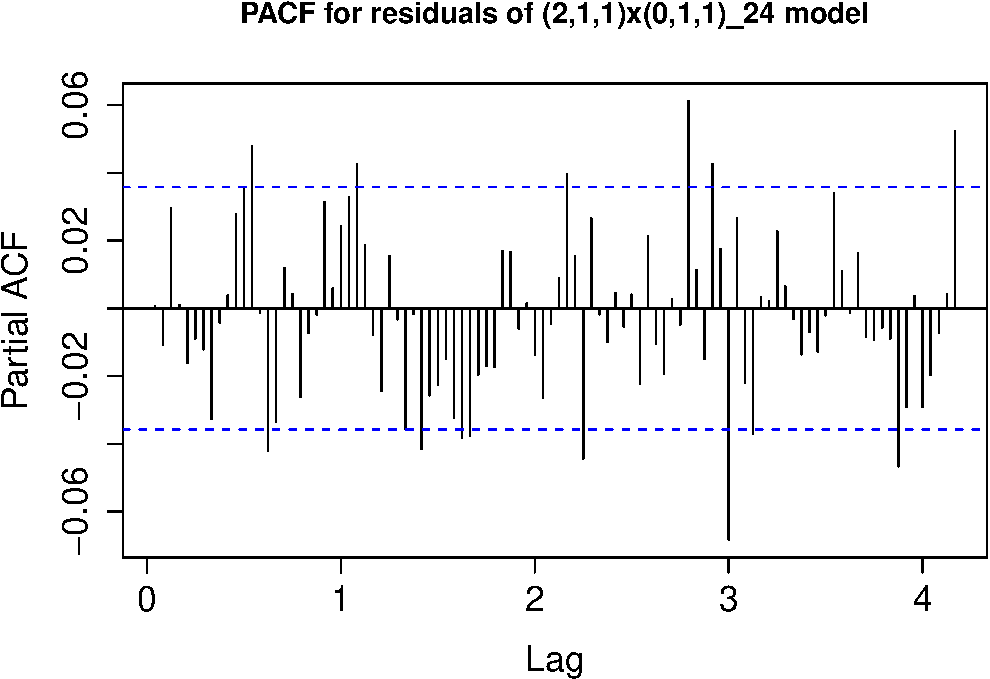
\includegraphics[width=70mm]{../plots/m21-residual-pacf.pdf}}}
    \parbox{.8\textwidth}{\lstinputlisting[firstline=5,lastline=10]{../tables/m21-summary.txt}}
    \caption{The \acf\ and \pacf\ for the residuals of the \mtwentyone\ model}
    \label{fig:m21-summary}
\end{figure}

It is seen that this model gives almost identical \acf\ and \pacf\ and the AIC-score has decreased. As the model is simpler than the previous models, this model\footnote{The even simpler \mnine\ model was also fitted (see \appref{m9}) but correlation begin to show for the first 5 lags.} is used as starting point for trying other seasonal ARMA-models.

\subsection*{The \mtwentytwo\ model}

The problem with the previous models is the high correlation at lag 72. Maybe it can be removed by increasing the order of the seasonal MA-part. The results from fitting the \mtwentytwo\ model is shown in figure~\ref{fig:m22-summary}.

\begin{figure}[!htb]
    \centering
    \mbox{\subfigure{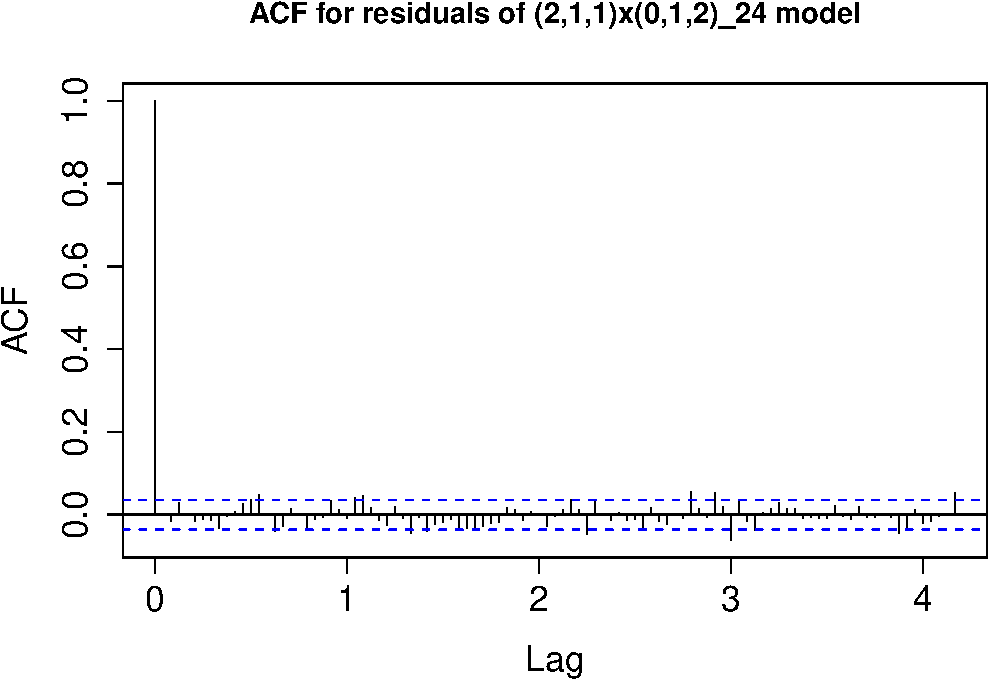
\includegraphics[width=70mm]{../plots/m22-residual-acf.pdf}} \quad 
          \subfigure{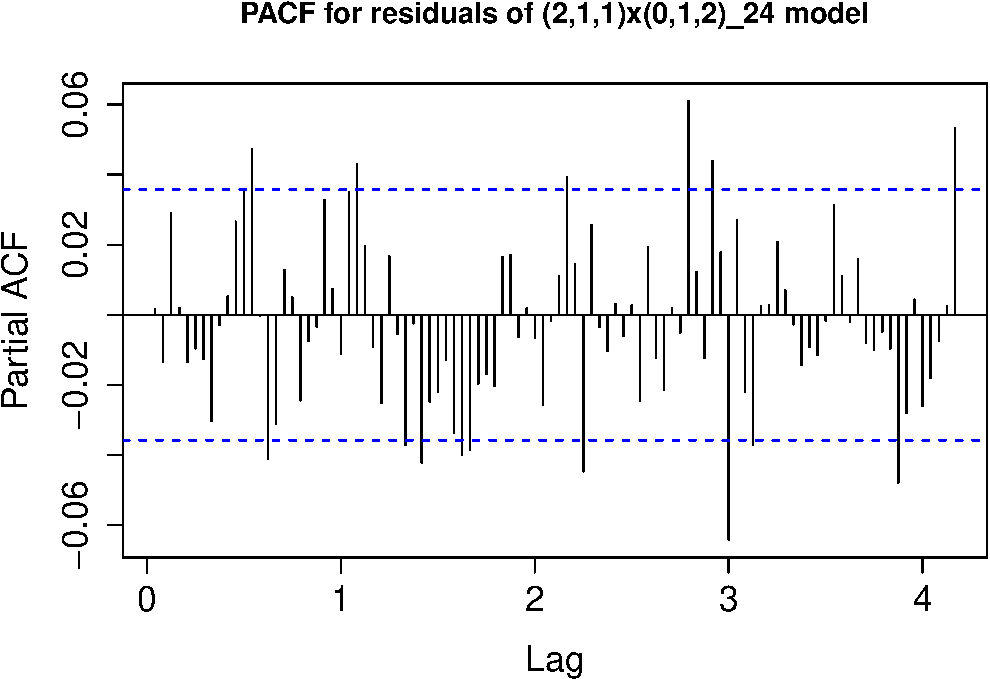
\includegraphics[width=70mm]{../plots/m22-residual-pacf.pdf}}}
    \parbox{.8\textwidth}{\lstinputlisting[firstline=5,lastline=10]{../tables/m22-summary.txt}}
    \caption{The \acf\ and \pacf\ for the residuals of the \mtwentytwo\ model}
    \label{fig:m22-summary}
\end{figure}

No progress is detected except for a slight decrease of the AIC score. The primary problem with high correlation at lag 72 remains. We try to increase the seasonal AR-part instead.

\subsection*{The \mtwentyeight\ model}

A model with an seasonal AR-part of order 1 is now fitted and the results are shown in figure~\ref{fig:m28-summary}.

\begin{figure}[!htb]
    \centering
    \mbox{\subfigure{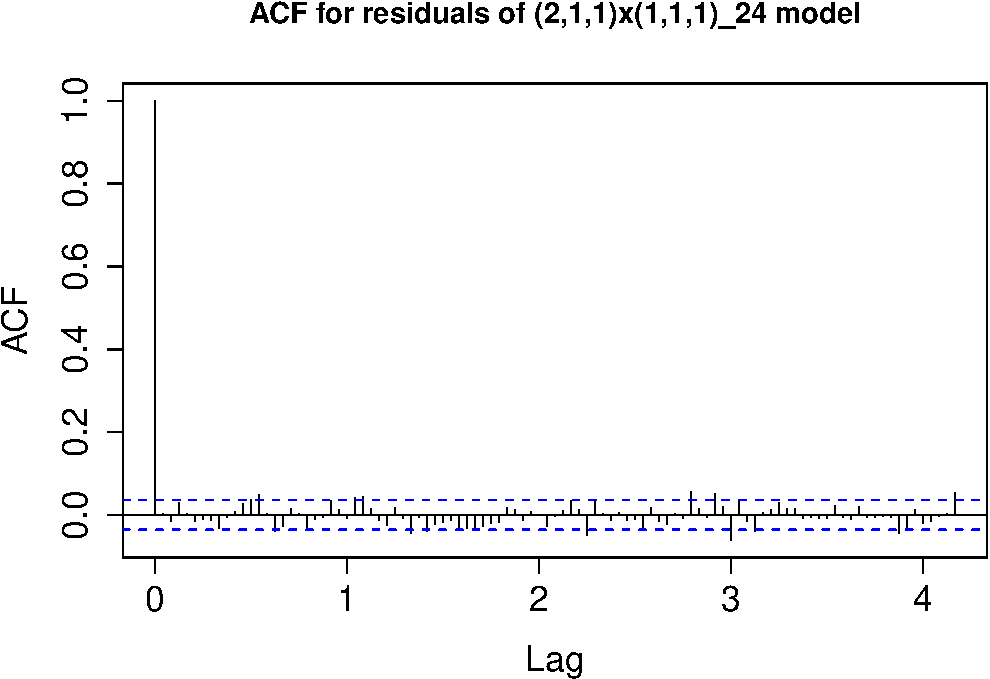
\includegraphics[width=70mm]{../plots/m28-residual-acf.pdf}} \quad 
          \subfigure{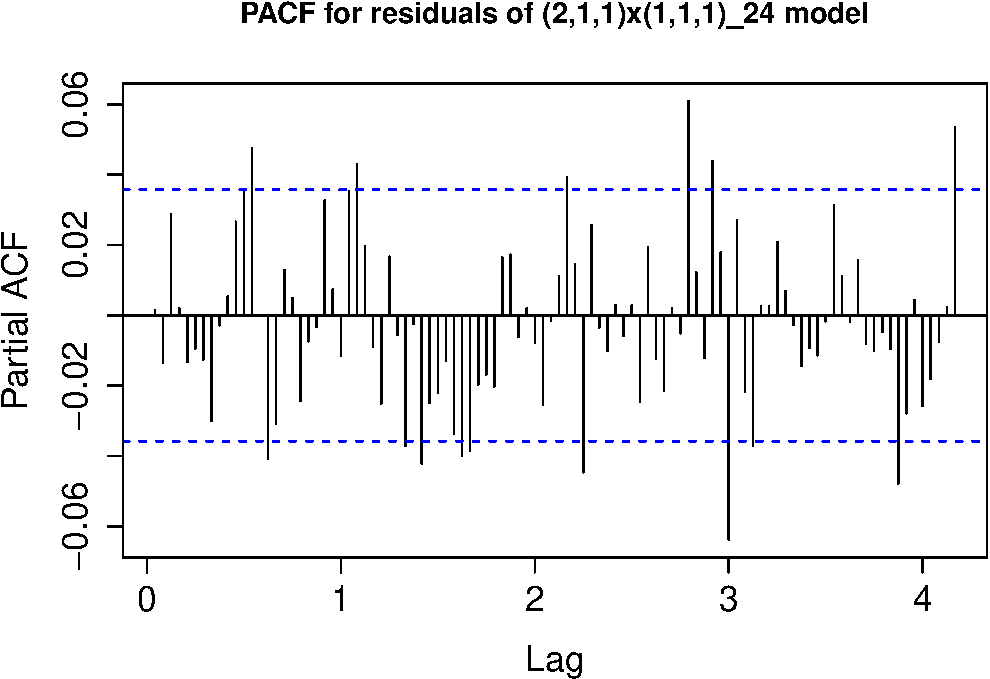
\includegraphics[width=70mm]{../plots/m28-residual-pacf.pdf}}}
    \parbox{.8\textwidth}{\lstinputlisting[firstline=5,lastline=10]{../tables/m28-summary.txt}}
    \caption{The \acf\ and \pacf\ for the residuals of the \mtwentyeight\ model}
    \label{fig:m28-summary}
\end{figure}

As usual no progress is detected, so another combination of the seasonal ARMA part should be tried. This is indeed what was done (see code in \appref{code-task1} for a complete list) but no model was found that was significantly better than the models already tried. Somehow there is some structure in the heat consumption series that is difficult to capture with a multiplicative seasonal model. Even though no model have been found that captures the structure perfectly, a model should be chosen to make predictions for one and six hours ahead. Apart from the \acf\ and the \pacf\ we should also make sign tests, Portmanteau test and QQ-plots for the different models. This is done in the code in \appref{code-task1} and the results for the different models are found to be close to each other\footnote{Since almost 30 models was tested all results isn't included in the appendices. See instead \githuburlfoot\ for all plots, tables etc}. 

\subsection*{Choosing \mtwentytwo\ as the final model}

Since many models performs almost identically, the choice of a final model is somewhat difficult. The \mtwentytwo\ model was chosen as the final model though, since it has one of the lowest AIC-score and all coefficients are significantly different from zero. To get a better picture of the model fit the output from the \myverb{tsdiag} function is shown in figure~\ref{fig:m22-tsdiag}.

\begin{figure}[!ht]
    \centering
    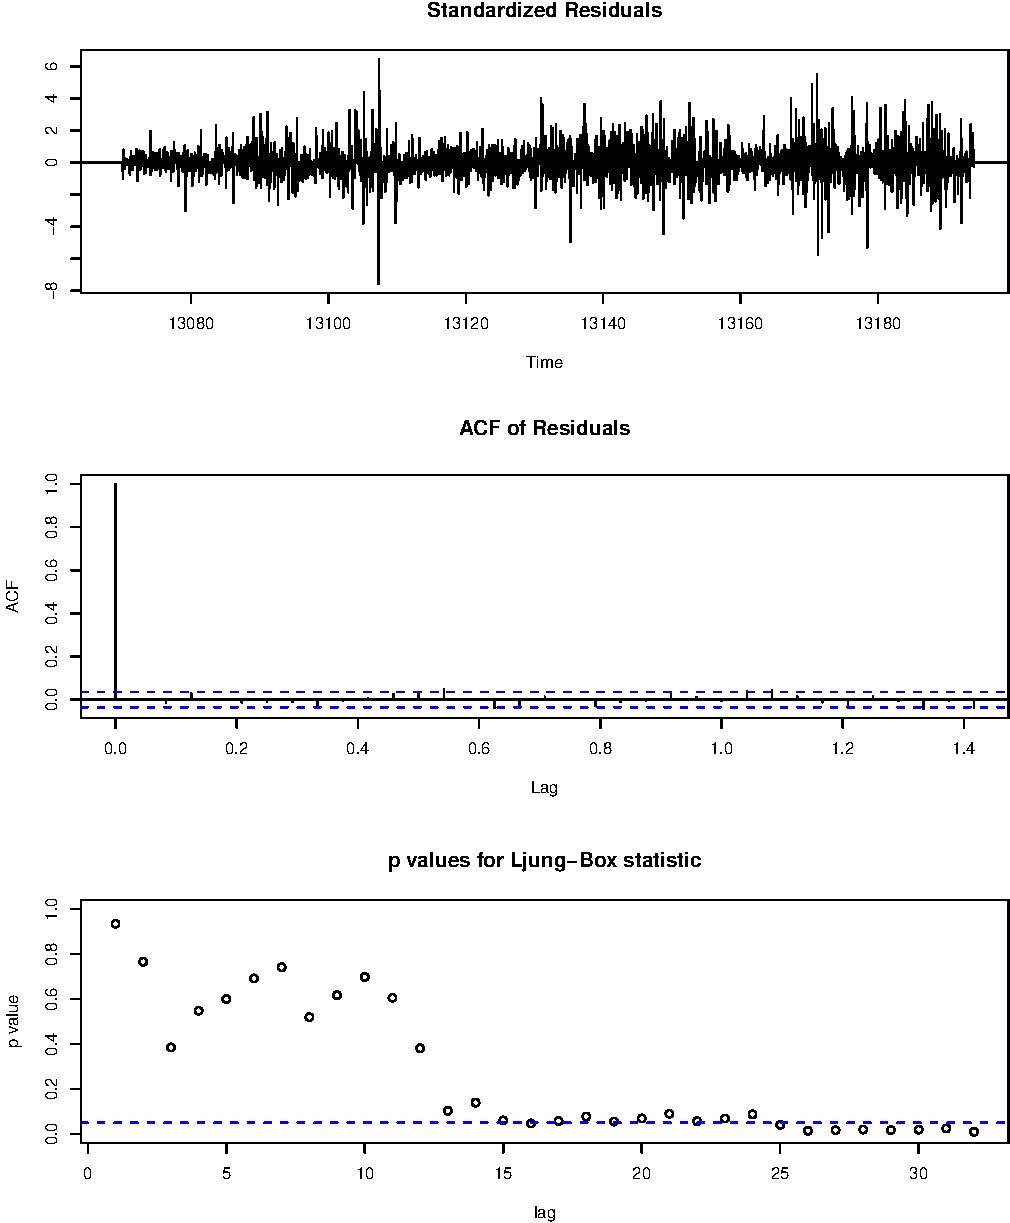
\includegraphics[width=90mm]{../plots/m22-tsdiag.pdf}
    \caption{Output from the \myverb{tsdiag} function for the \mtwentytwo\ model}
    \label{fig:m22-tsdiag}
\end{figure}

From the \myverb{tsdiag} it is seen that the Portmanteau test (Ljung-Box is just an adjusted Portmanteau test) shows significantly deviations from a chi squared distribution when lags larger than 15 are included in the sum of squares of residual autocorrelation values. It reinforce that there is some seasonal structure that isn't captured by the chosen model. One possibility is that there is a second seasonallity with another period than 24. This won't be examined further in this report, but it could be worth investigating.

The model also do not pass the sign test. The p-value is $3.8\cdot 10^{-8}$.

Apart from the \myverb{tsdiag} plot and the sign test, a QQ-plot of the residuals is also created and shown in figure~\ref{fig:m22-qq}. It is seen that the residual distribution is more heavy tailed than a normal distribution. This is expected when a model don't fit the data well since the residuals will tend to be larger than ``expected''. This is worth remembering when we now turn to prediction and confidence intervals for the predictions.

\begin{figure}[!ht]
    \centering
    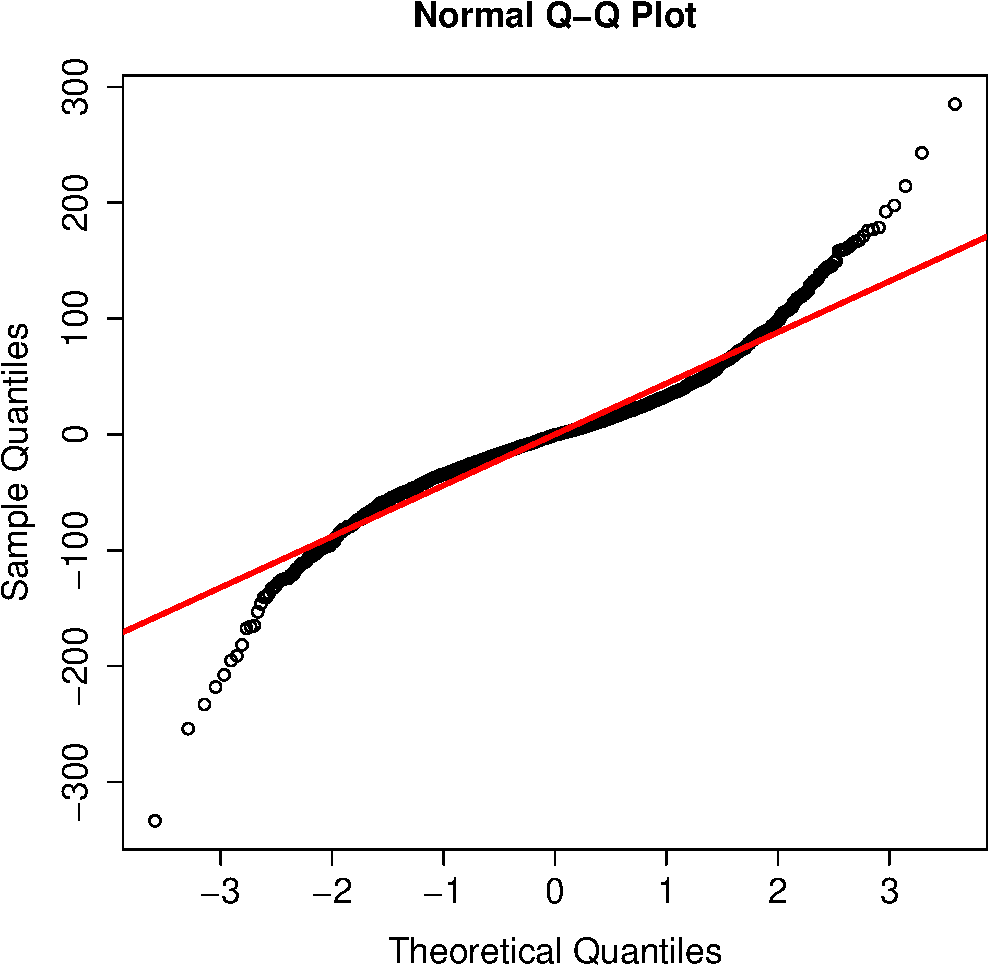
\includegraphics[width=90mm]{../plots/m22-qq.pdf}
    \caption{QQ-plot for the \mtwentytwo\ model}
    \label{fig:m22-qq}
\end{figure}

\subsection*{Predicting 6 hours ahead with the \mtwentytwo\ model}

The heat consumption 1 and 6 hours ahead should now be predicted. The relevant theory is described in section 5.7.1 in \cite{hm} but the predictions, and the corresponding confidence intervals, are calculated using the \myverb{predict} function in R. The predictions 6 hours ahead are shown in figure~\ref{fig:m22-predictions} and the values are given in table~\ref{tbl:m22-predictions}.

\begin{figure}[ht]
    \centering
    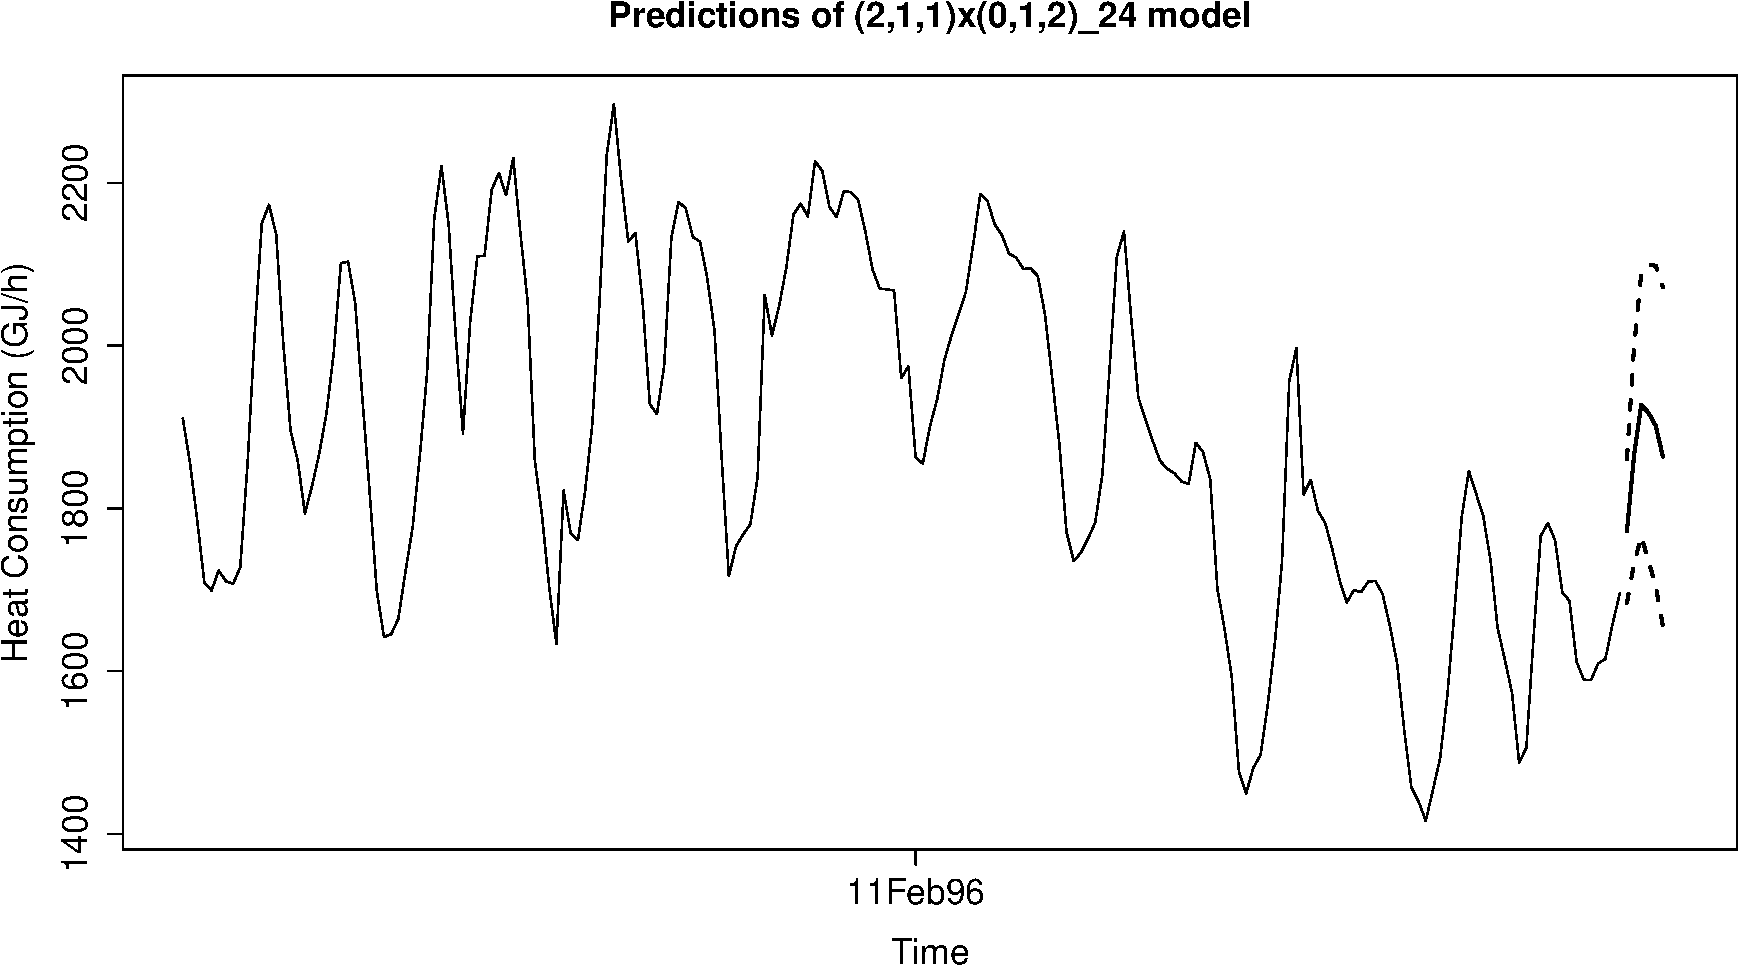
\includegraphics[width=120mm]{../plots/m22-predictions.pdf}
    \caption{Predictions of \mtwentytwo\ model}
    \label{fig:m22-predictions}
\end{figure}

\begin{table}
    \centering
    \begin{tabular}{c c c c}
        Time ahead & Prediction & Error & Interval \\\hline
1 & 1772.05 & 86.38 & [1685.67; 1858.43]\\
2 & 1865.74 & 130.24 & [1735.50; 1995.99]\\
3 & 1927.45 & 158.65 & [1768.79; 2086.10]\\
4 & 1917.34 & 178.21 & [1739.13; 2095.55]\\
5 & 1901.66 & 192.56 & [1709.10; 2094.21]\\
6 & 1863.67 & 203.70 & [1659.97; 2067.37]

    \end{tabular}
    \caption{Predictions of \mtwentytwo\ model}
    \label{tbl:m22-predictions}
\end{table}

Both from the plot and the table of the predicted values it is seen how the uncertainty in the predictions increases as the time gets futher into the future. Already for 6 hours into the future the uncertainty so large that the prediction may be almost useless. It is also worth noticing that the calculated 95\% prediction interval do not include the uncertainty in the estimated model parameters. The actual confidence interval will therefore be larger than what is shown in the plot and table.


\section*{Building the complex model}

In the previous section we had trouble finding a suitable model describing the heat consumption data. In this section we will try to incorporate additional climate data in the model. By including this extra information we hope to build a better model. Specifically we have 3 extra time series with hourly measurements of Ambient Air Temperature, the Wind Speed and the Global Radiation for the same time period as the heat consumption measurements. To build a good model it should be determined which of the climate time series that are correlated with the heat consumption time series.

\subsection*{Estimating cross correlation functions}

The estimated cross correlation function (CCF) between two time series is given by equation 6.17 in \cite{hm}. Unfortunately the estimated cross correlation function may show significant correlations even for two uncorrelated series. The time series therefore needs to be pre-whitened before calculating the CCF. The pre-whitening and estimation of the CCF is done by the \myverb{prewhiten} function from the package \myverb{TSA}. Using this function the CCF is calculated for the combination of the heat consumption series and the three climate series. The result is shown in figure~\ref{fig:ccfs}

\begin{figure}
    \centering
    \mbox{\subfigure{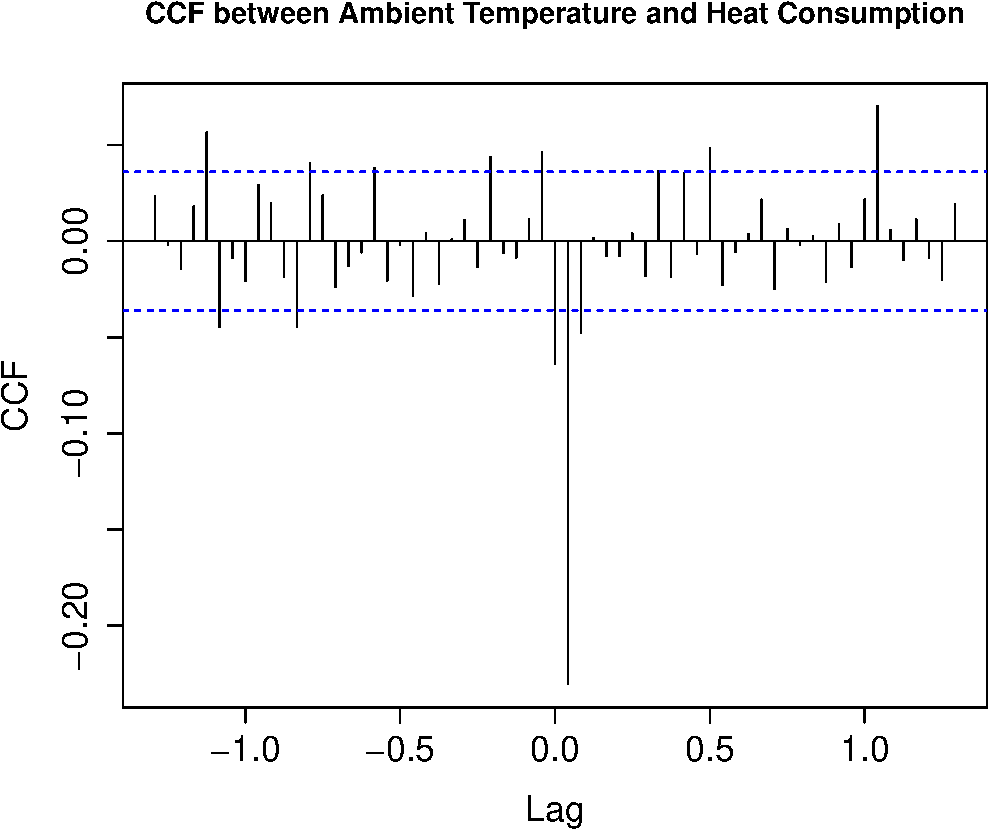
\includegraphics[width=50mm]{../plots/ta-ccf.pdf}} \quad 
        \subfigure{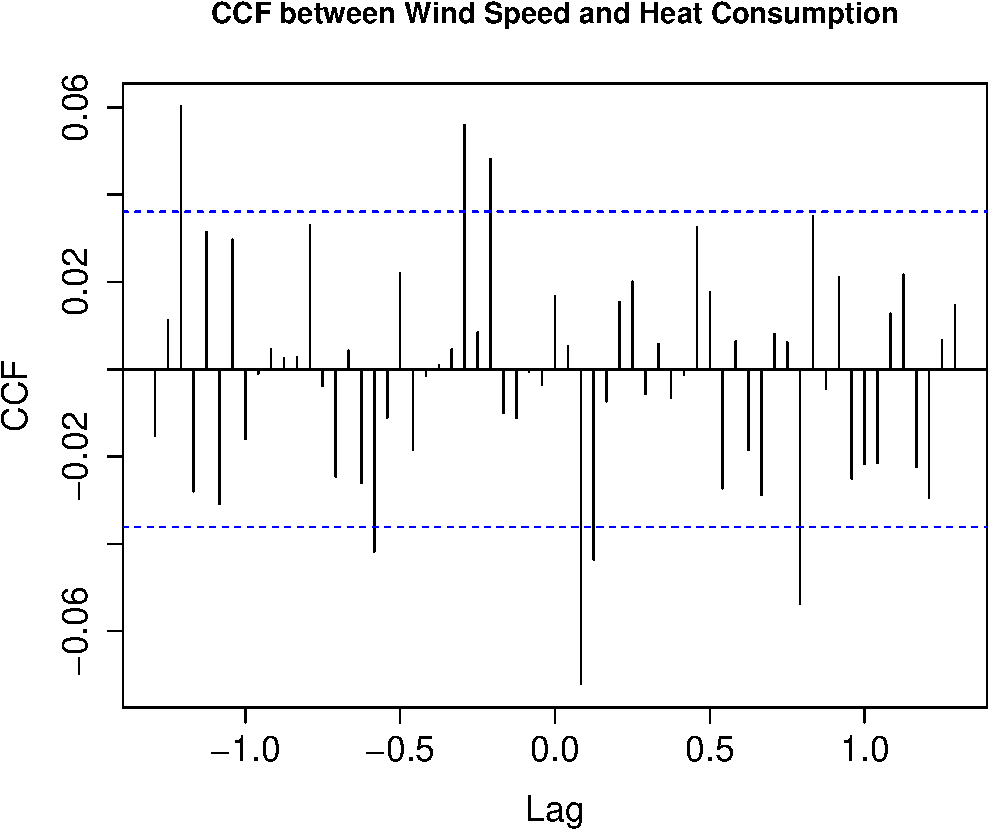
\includegraphics[width=50mm]{../plots/w-ccf.pdf}}\quad 
        \subfigure{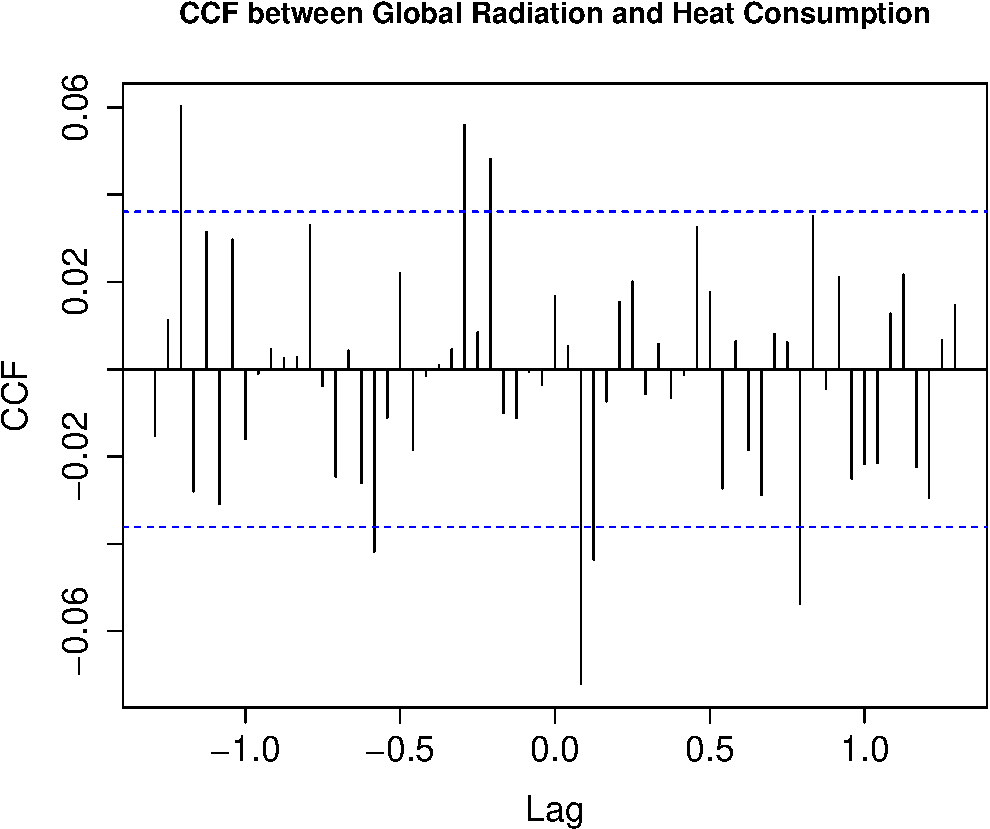
\includegraphics[width=50mm]{../plots/gr-ccf.pdf}}}
    \caption{CCFs for the Heat Consumption data and the three different climate time series}
    \label{fig:ccfs}
\end{figure}

From the figure it is seen that the CCF with the largest correlation values is the CCF between the ambient temperature and the heat consumption. From the plot it is seen that approximately $\rho_{\epsilon\alpha}(1)\approx -0.22$ where $\epsilon$ is the white noise from the temperature series and $\alpha$ is the ``white noise'' of the heat consumption series. The interpretation is that increasing temperature results in less heat consumption the next hour, which seems quite sensible.

\subsection*{Using the Ambient Temperature as exogenous input}

A model that includes the ambient temperature as an exogenous variable is now created. The model order is still given as \mtwentytwo. Using the \myverb{arima} function the model parameters are estimated and gives the model summary and residual \acf/\pacf\ shown in figure~\ref{fig:tfm1-summary}

\begin{figure}[!htb]
    \centering
    \mbox{\subfigure{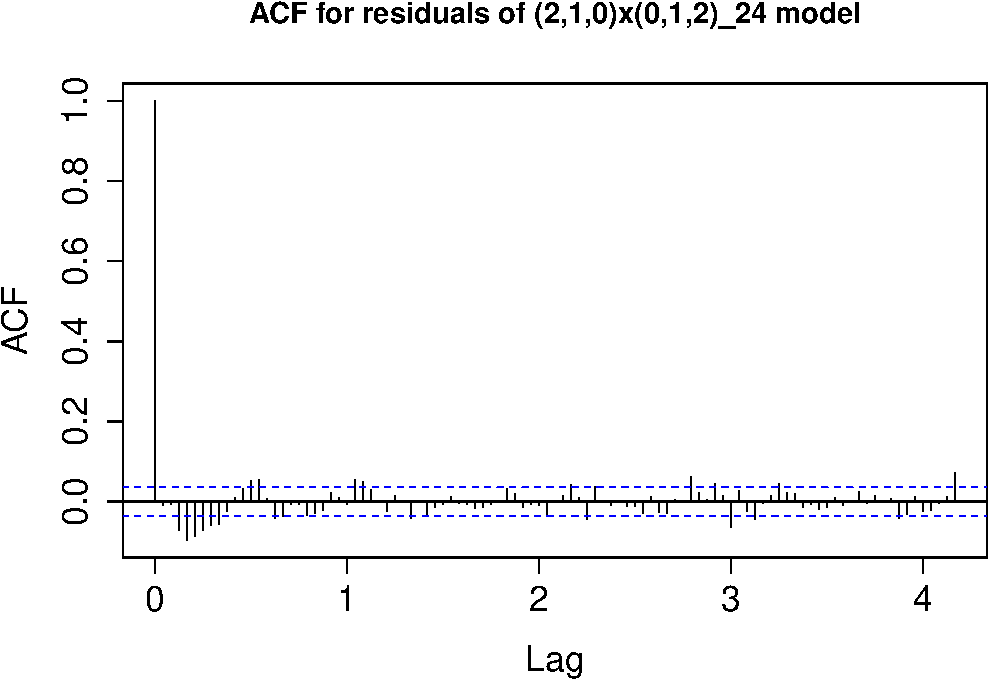
\includegraphics[width=70mm]{../plots/tfm1-residual-acf.pdf}} \quad 
          \subfigure{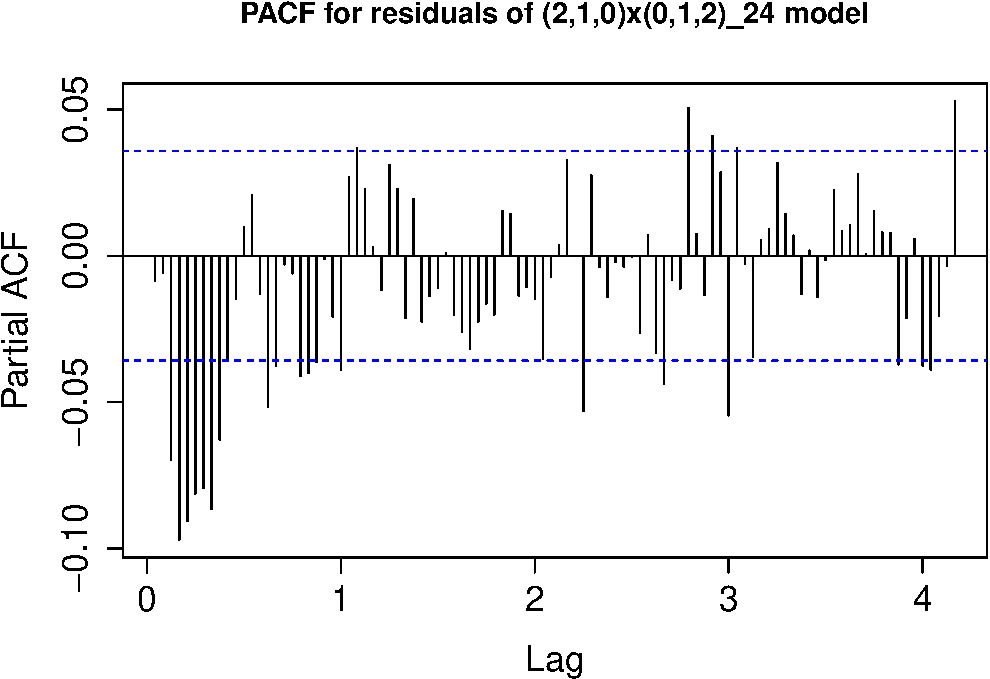
\includegraphics[width=70mm]{../plots/tfm1-residual-pacf.pdf}}}
    \parbox{.8\textwidth}{\lstinputlisting[firstline=5,lastline=10]{../tables/tfm1-summary.txt}}
    \caption{Summary for the \mtwentytwo\ transfer model}
    \label{fig:tfm1-summary}
\end{figure}

Although the AIC score has decreased a higher correlation is seen in the residuals for the first 6 lags. All parameters are seen to be significant and maybe a better model could be obtained by raising the non-seasonal ARIMA order. Therefore a \tfmtwo\ is fitted to the data, still with the ambient temperature as exogenous input. The results are shown in figure~\ref{fig:tfm2-summary}.

\begin{figure}[!htb]
    \centering
    \mbox{\subfigure{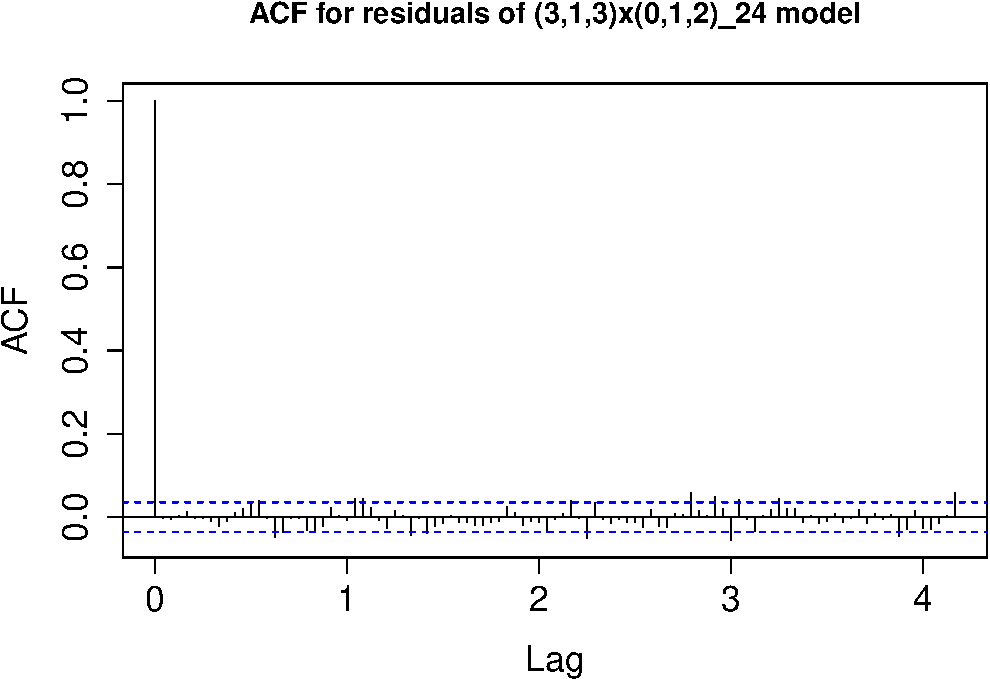
\includegraphics[width=70mm]{../plots/tfm2-residual-acf.pdf}} \quad 
          \subfigure{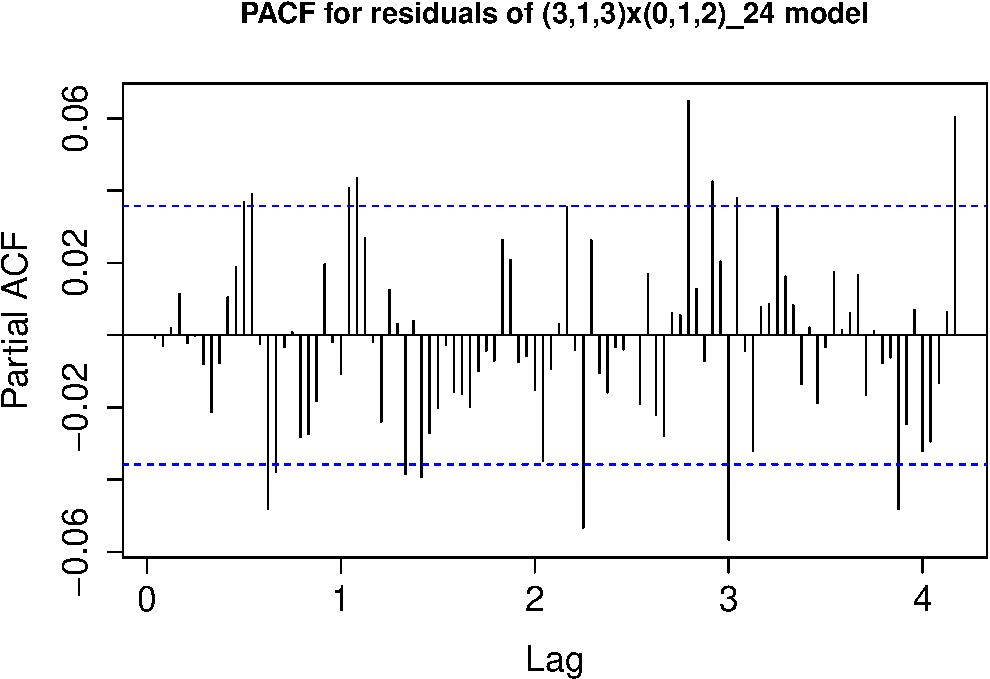
\includegraphics[width=70mm]{../plots/tfm2-residual-pacf.pdf}}}
    \parbox{.8\textwidth}{\lstinputlisting[firstline=5,lastline=13]{../tables/tfm2-summary.txt}}
    \caption{Summary for the \tfmtwo\ transfer model}
    \label{fig:tfm2-summary}
\end{figure}

The AIC score has decreased further and the high correlation for lags below 6 has disappeared. The \pacf\ still shows the same structure as for the model without the temperature series as input. Allthough the model should be further refined we accept it for now, and look at some of the other model checks. In figure~\ref{fig:tfm2-tsdiag}

\begin{figure}[ht]
    \centering
    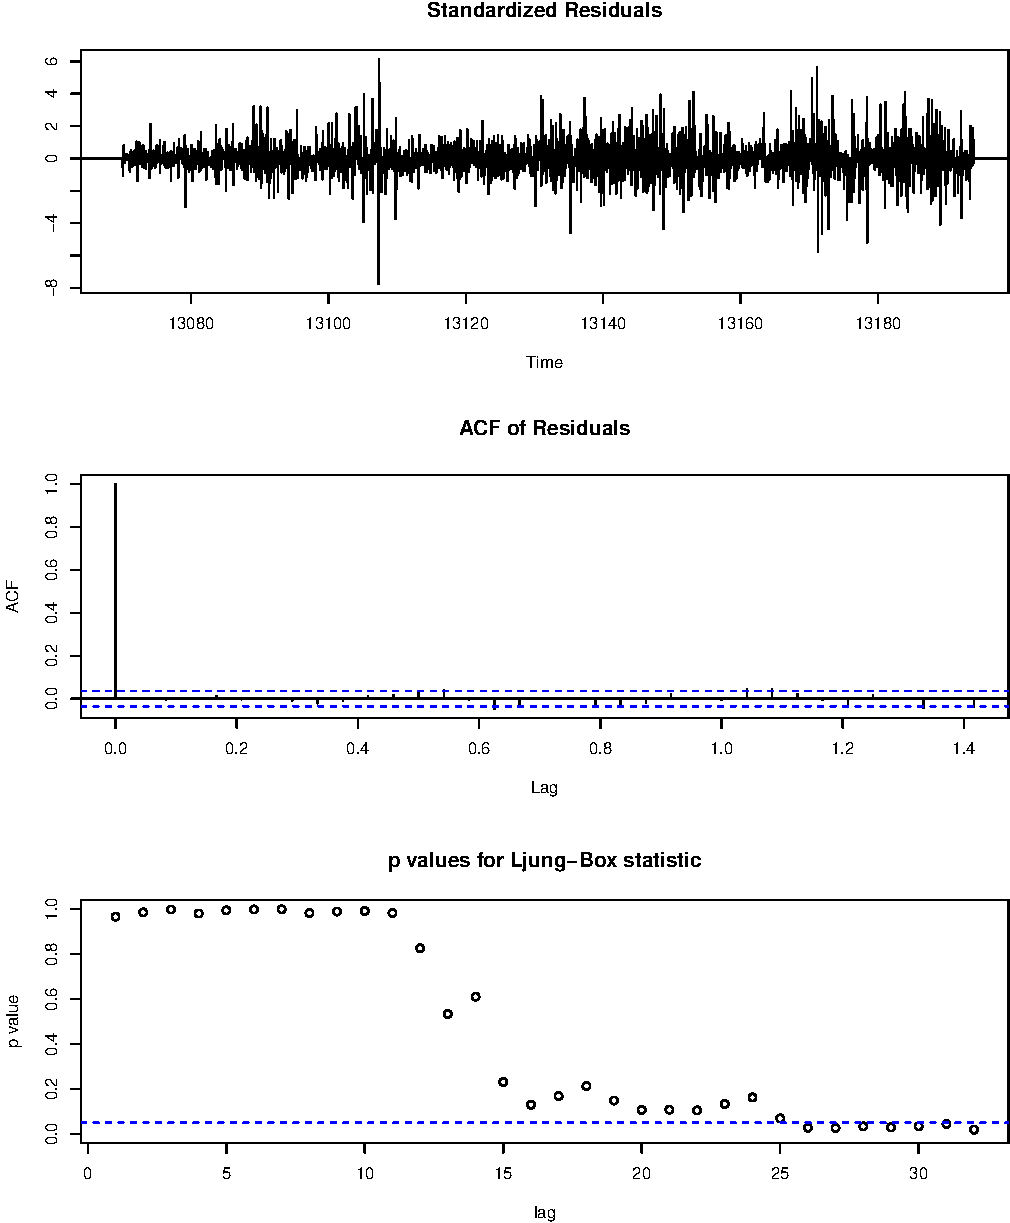
\includegraphics[width=90mm]{../plots/tfm2-tsdiag.pdf}
    \caption{Output from the \myverb{tsdiag} function for the \tfmtwo\ transfer model}
    \label{fig:tfm2-tsdiag}
\end{figure}

Generally it is the same structure as for the model without extra input. Although for lags between 15 and 25 the model with extra input has slightly higher p-values for the Portmanteau test. A sign test for the residuals gives a p-value of 3.3\% which is much better than for the simple model. The QQ-plot for the residuals is shown in figure~\ref{fig:tfm2-qq} and it looks almost completely identical with the QQ plot for the simple model.

\begin{figure}[!ht]
    \centering
    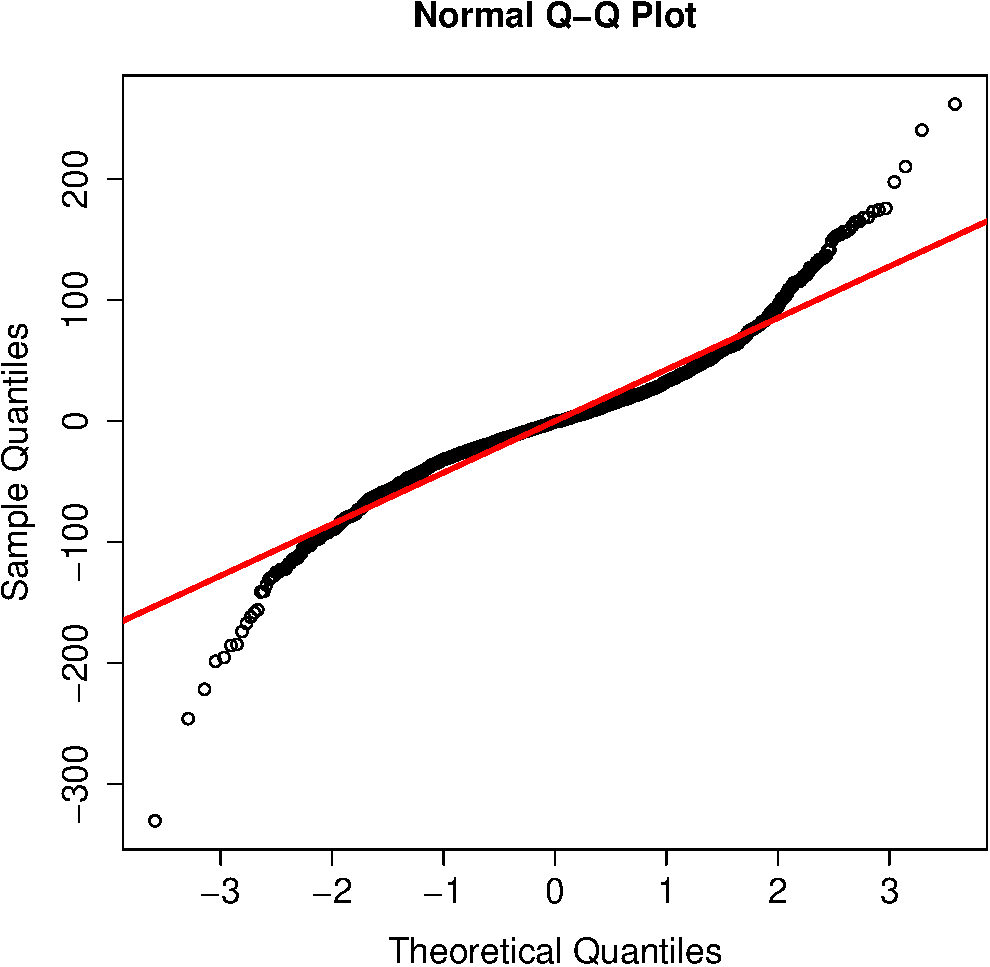
\includegraphics[width=90mm]{../plots/tfm2-qq.pdf}
    \caption{QQ plot for the \tfmtwo\ transfer model}
    \label{fig:tfm2-qq}
\end{figure}

\FloatBarrier

\subsection*{Prediting with the \tfmtwo\ model with exogenous input}

We are now ready to make predictions with the found model. The 6 step ahead predictions are shown in figure~\ref{fig:tfm2-predictions}

\begin{figure}[!ht]
    \centering
    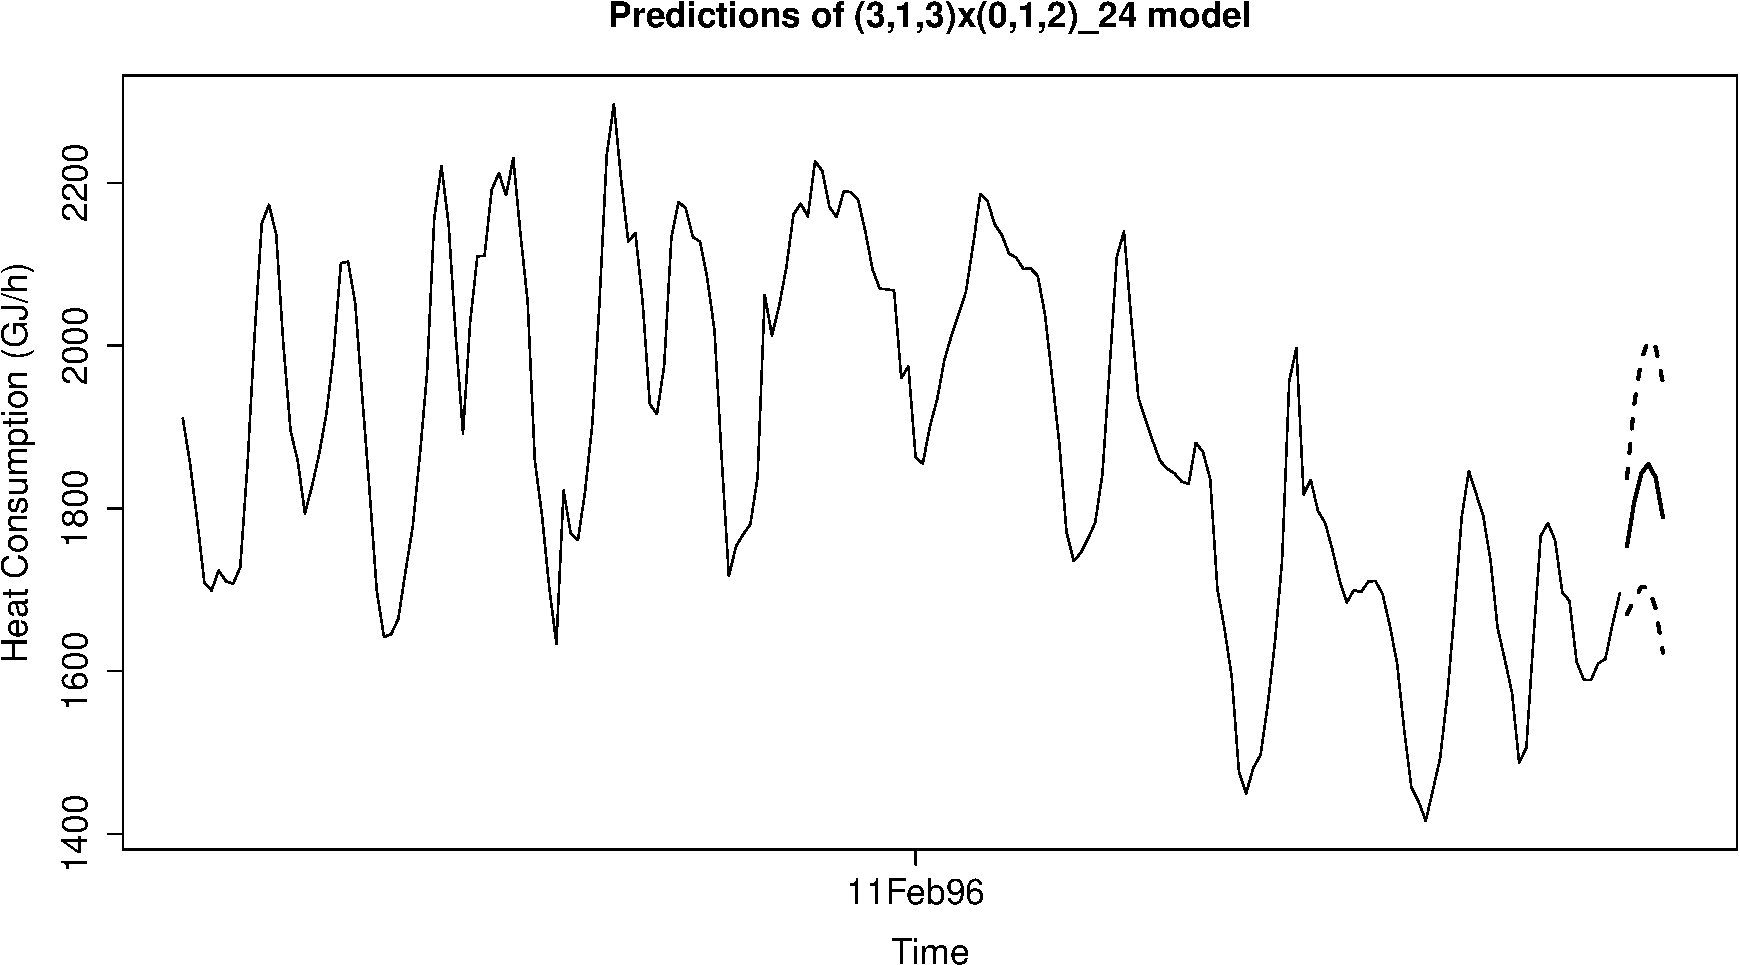
\includegraphics[width=120mm]{../plots/tfm2-predictions.pdf}
    \caption{Predictions from the \tfmtwo\ transfer model}
    \label{fig:tfm2-predictions}
\end{figure}

\FloatBarrier

\pagebreak

\renewcommand\thesection{\Alph{section}}
\section{Appendices}

All R code used for this assignment is included here. All source code incl.
latex code for this report can be found at \githuburl


%\subsection{Load data script}
%\lstinputlisting{../src/loaddata.R}

\subsection{Results for the \mten and \meleven model}\label{app:m10-m11}
\begin{figure}[!htb]
    \centering
    \mbox{\subfigure{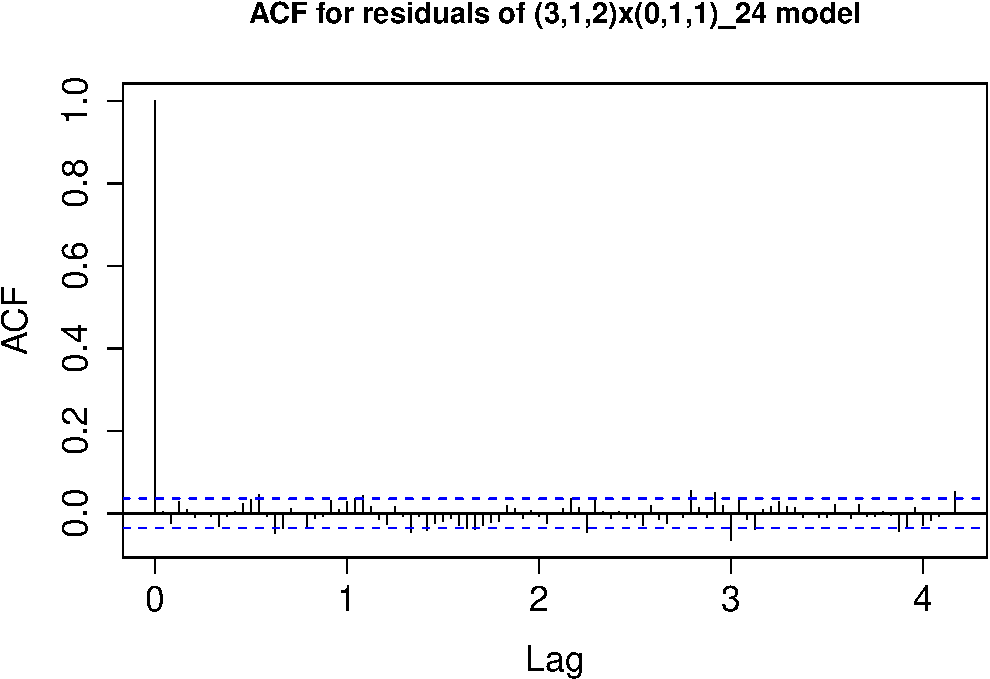
\includegraphics[width=70mm]{../plots/m10-residual-acf.pdf}} \quad 
          \subfigure{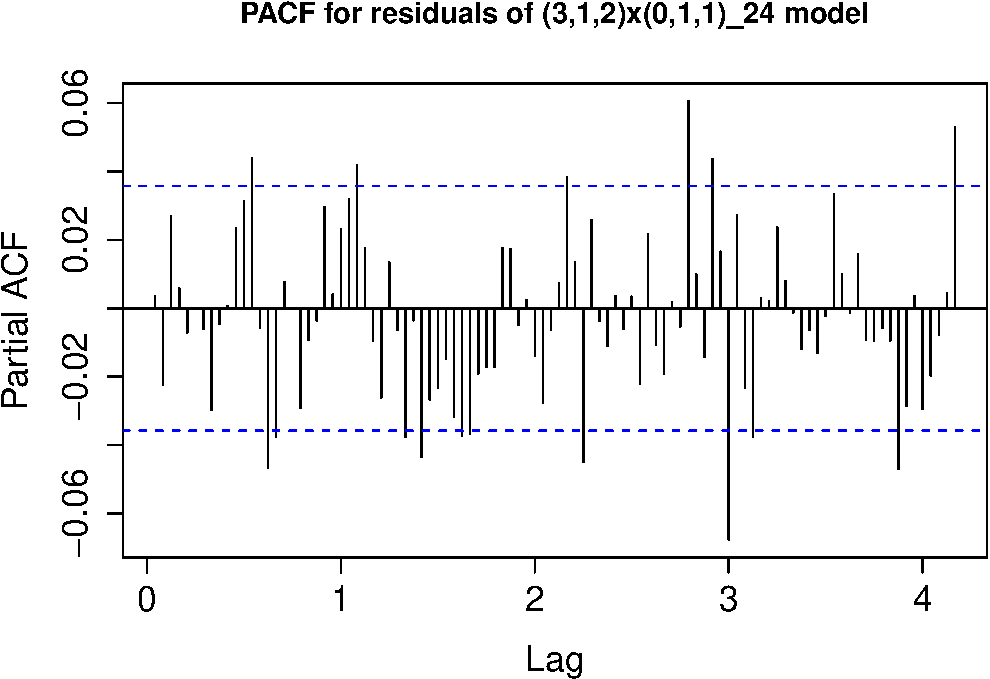
\includegraphics[width=70mm]{../plots/m10-residual-pacf.pdf}}}
    \parbox{.8\textwidth}{\lstinputlisting[firstline=5,lastline=10]{../tables/m10-summary.txt}}
    \caption{Summary for the \mten\ model}
    \label{fig:m10-summary}
\end{figure}
\begin{figure}[!htb]
    \centering
    \mbox{\subfigure{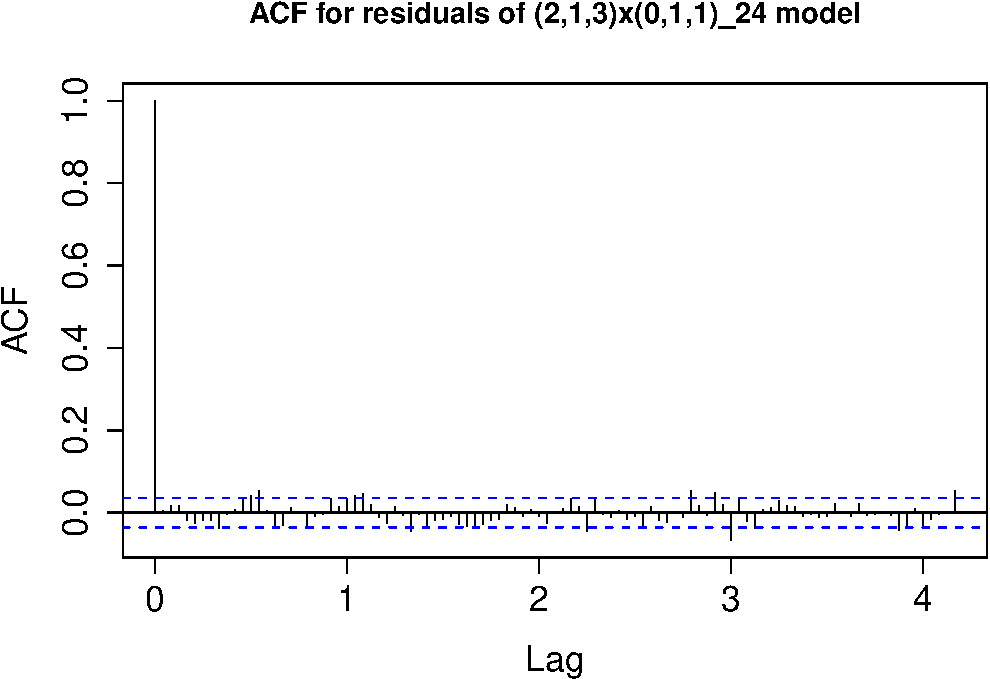
\includegraphics[width=70mm]{../plots/m11-residual-acf.pdf}} \quad 
          \subfigure{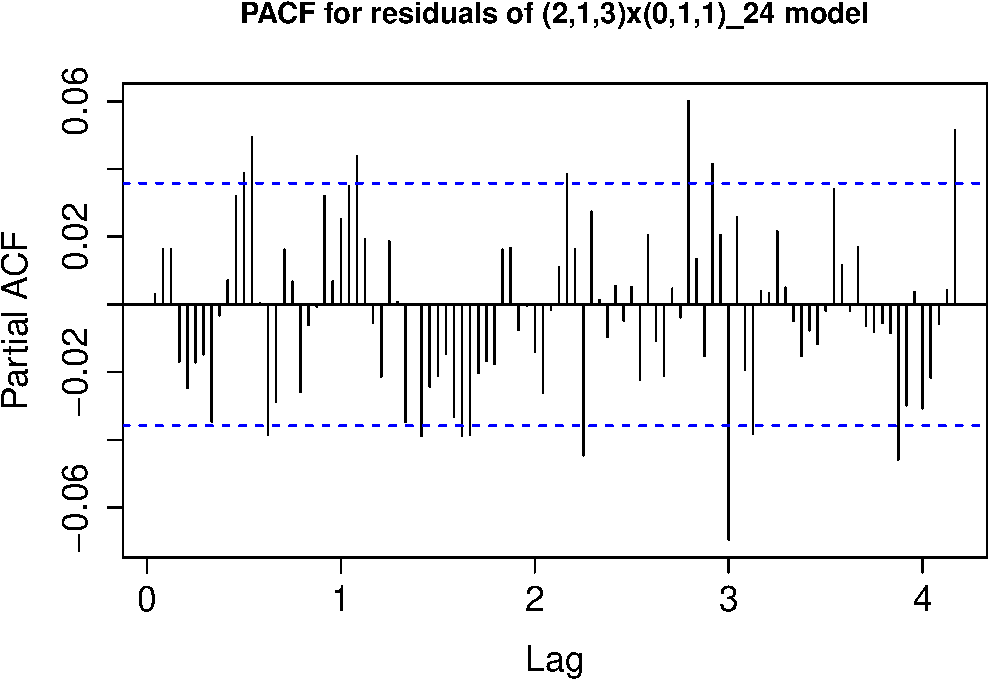
\includegraphics[width=70mm]{../plots/m11-residual-pacf.pdf}}}
    \parbox{.8\textwidth}{\lstinputlisting[firstline=5,lastline=10]{../tables/m11-summary.txt}}
    \caption{Summary for the \meleven\ model}
    \label{fig:m11-summary}
\end{figure}

\FloatBarrier

\subsection{Results for the \mnine\ model}\label{app:m9}
\begin{figure}[!htb]
    \centering
    \mbox{\subfigure{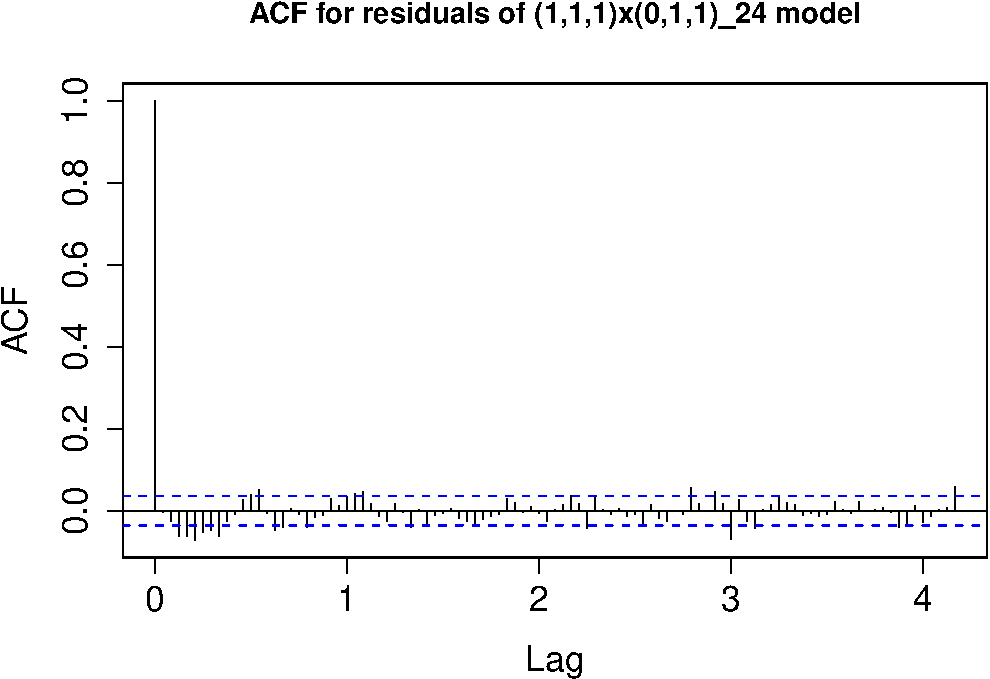
\includegraphics[width=70mm]{../plots/m9-residual-acf.pdf}} \quad 
          \subfigure{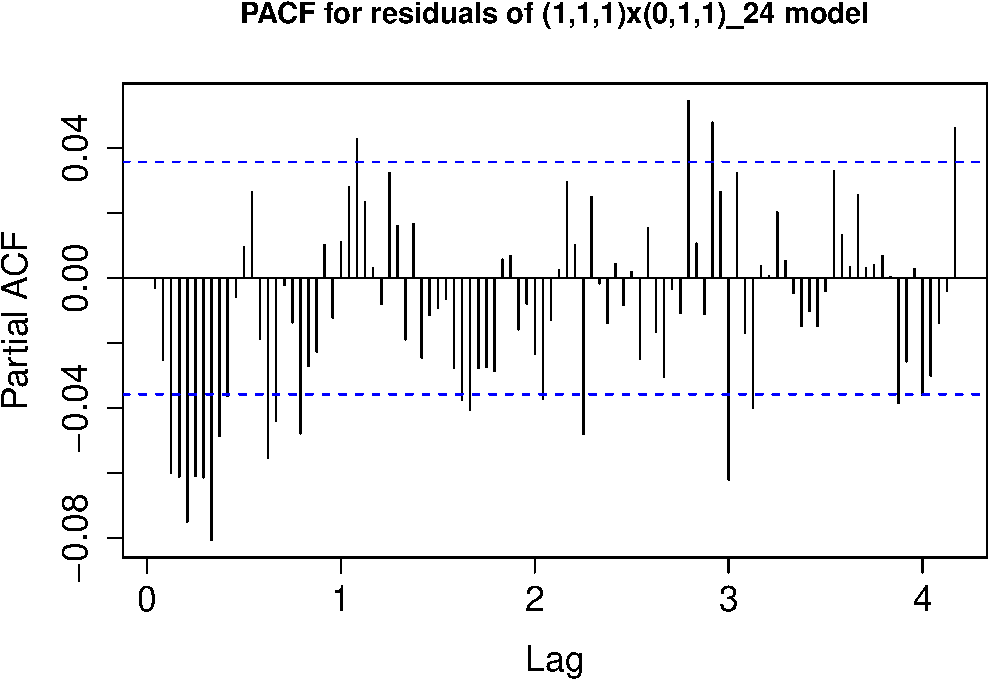
\includegraphics[width=70mm]{../plots/m9-residual-pacf.pdf}}}
    \parbox{.8\textwidth}{\lstinputlisting[firstline=5,lastline=10]{../tables/m9-summary.txt}}
    \caption{Summary for the \mnine\ model}
    \label{fig:m9-summary}
\end{figure}


\subsection{Loading data}\label{app:code-loaddata}
\lstinputlisting{../src/loaddata.R}

\subsection{R code for task 1 and task 2}\label{app:code-task1}
\lstinputlisting{../src/task1.R}

\subsection{R code for task 3 and task 4}\label{app:code-task3}
\lstinputlisting{../src/task2.R}

\subsection{Helper functions}\label{app:code-helpers}
\lstinputlisting{../src/functions.R}

\pagebreak

\begin{thebibliography}{9}

\bibitem{hm}
  Henrik Madsen,
  \emph{Time Series Analysis}.
  Chapman \& Hall/CRC,
  1st Edition,
  2008.

%\bibitem{taleb}
%  Nassim Nicholas Taleb,
%  \emph{The Black Swan}.
%  Random House Trade Paperbacks
%  2nd Edition,
%  2010.

\end{thebibliography}


\end{document}
